\chapter{Metodolog\'ia de evaluaci\'on}
\label{chap:metodologia}
%mostrar métricas, explicar VI brevemente, explicar que no es necesario Structure-Aware rand index ya que los caminos p subconjunto de P', p pertenece P, cumplen por si solos en ser soluciones factibles de segmentos de filamento y que la unión de caminos para formar un filamento, al cumplir con las restricciones también genera solo filamentos factibles
% Dado que Rand y  Jaccard vienen de valores extraidos desde la contingency table, es posible obtener información útil de la mano de precisión, recall y F1

Al basar la individualizaci\'on de filamentos en un m\'etodo que usa un grafo, el resultado obtenido es un conjunto de caminos, donde cada camino es a su vez un conjunto de aristas. El proceso de individualizar filamentos genera una partici\'on o {\it clustering} del grafo, donde las aristas corresponden al {\it data set}, con cada camino representando a un cluster perteneciente al clustering. La partici\'on propuesta por un m\'etodo basado en grafos debe ser comparada con respecto a la partici\'on generada por un experto, a la que nos referiremos como {\it ground truth}. Uno de los requisitos de esta comparaci\'on, es que ambas particiones se refieran al mismo data set, lo que implica que ambas deben realizarse en base al mismo grafo. Adem\'as se debe considerar que el clustering realizado por el experto puede tener una cantidad igual o distinta de clusters con respecto al clustering producido por el m\'etodo a evaluar.



\section{M\'etricas y Medidas}
\label{sec:metricasymedidas}


La comparaci\'on de particiones en donde una corresponde al {\it ground truth} implica que las mediciones a utilizar son del tipo de criterio externo \cite{manning20introduction}. En este tipo de criterio hay \'indices basados en comparaci\'on mediante conteo de pares, como el \'indice {\it Rand} ($\mathcal{R}$), el \'indice {\it Jaccard} ($\mathcal{J}$), y la medida $\mathcal{F}$ tambi\'en conocida como $F1-$Score. Por otra parte, tambi\'en existen m\'etricas del \'area de teor\'ia de la informaci\'on como {\it Variation of Information} o VI para el mismo prop\'osito. Estos m\'etodos ser\'an la base de comparaci\'on de particiones en esta investigaci\'on.

\subsection{\'Indices Rand y Jaccard}

La mayor\'ia de los criterios para comparar particiones mediante conteo de pares suele fundamentarse en el uso de la matriz de confusi\'on, tambi\'en llamada matriz de asociaci\'on o tabla de contingencia \cite{meilua2007comparing}. Esta tabla considera 4 casos en los que puede estar un par de elementos del {\it data set}, que para el caso de la individualizaci\'on de filamentos son pares de aristas, en las particiones $C$ y $C'$:

\begin{itemize}
    \item $N_{11}$: N\'umero de pares que est\'an en el mismo cluster en $C$ y $C'$
    \item $N_{00}$: N\'umero de pares que est\'an en distintos clusters en $C$ y $C'$
    \item $N_{10}$: N\'umero de pares que est\'an en el mismo cluster en $C$ pero no en $C'$
    \item $N_{01}$: N\'umero de pares que est\'an en el mismo cluster en $C'$ pero no en $C$
\end{itemize}

Se tiene que $N_{11} + N_{00} + N_{10} + N_{01} = \frac{n(n-1)}{2}$, con n como el n\'umero de aristas.

Lo definici\'on de los casos utilizados para formar la tabla de contingencia posibilita asociar cada caso con una correspondiente evaluaci\'on de clasificaci\'on como se indica en la tabla \ref{tab:EquivParesClasificacion}.

\begin{table}[h]
    \centering
    \begin{tabular}{|c|c|}
    \hline
        Casos para un par de aristas & Clasificaci\'on \\ \hline
        $N_{11}$ & Verdadero Positivo ({\it True Positive} o TP) \\
        $N_{00}$ & Verdadero Negativo ({\it True Negative} o TN)\\
        $N_{10}$ & Falso Positivo ({\it False Positive} o FP)\\
        $N_{01}$ & Falso Negativo ({\it False Negative} o FN)\\ \hline
    \end{tabular}
    \caption{Equivalencia entre casos para un par de aristas con su respectiva clasificaci\'on}
    \label{tab:EquivParesClasificacion}
\end{table}

La ecuaci\'on \ref{eq:randIndex} expresa que el \'indice Rand puede ser escrito en funci\'on de evaluaciones de clasificaci\'on, lo que lo hace coincidir con la definici\'on de la medida de exactitud ({\it Accuracy}). $\mathcal{R}$ adquiere el valor 0 para particiones totalmente diferentes, subiendo hasta llegar a 1, lo que indica que las particiones son id\'enticas. Algunas cr\'iticas al \'indice Rand se\~nalan la alta sensibilidad que tiene al valor de TN, el que tiende a ser mucho mayor que el resto \cite{ben2001stability}, la existencia de una alta dependencia al n\'umero de clusters \cite{wagner2007comparing}, y que los valores de $\mathcal{R}$ tienden a concentrarse en un intervalo cerca de 1, puntualmente en el rango [0.5, 1] \cite{meilua2007comparing}\cite{vinh2010information}.

\begin{equation}
\mathcal{R}(C,C^{\prime}) = \frac{N_{11} + N_{00}}{n(n-1)/2} = \frac{TP + TN}{TP + TN + FP + FN}
\label{eq:randIndex}
\end{equation}

Por su parte, el \'indice Jaccard es similar al \'indice Rand con la excepci\'on que ignora la clasificaci\'on TN, como se observa en la ecuaci\'on \ref{eq:JaccardIndex}. Su valor tambi\'en oscila entre 0 y 1 para particiones totalmente distintas y particiones id\'enticas respectivamente. Una de las cr\'itica es que puede entregar resultados no confiables para data sets muy peque\~nos.

\begin{equation}
\mathcal{J}(C,C^{\prime}) = \frac{N_{11}}{N_{11} + N_{01} + N_{10}} = \frac{TP}{TP + FP + FN}
\label{eq:JaccardIndex}
\end{equation}

La ventaja que presentan $\mathcal{R}$ y $\mathcal{J}$ sobre VI radica en que estos \'indices si pueden considerar casos de superposici\'on.

\subsection{Variation of Information}
La m\'etrica VI definida en \cite{meilua2007comparing} se fundamenta en la informaci\'on asociada a la entrop\'ia de las particiones a comparar, as\'i como en la informaci\'on mutua que comparten. El rango de valores de VI comienza en 0 para 2 particiones iguales, llegando a $\log n$ para particiones absolutamente distintas, con $n$ como el n\'umero de elementos del data set. En la ecuaci\'on \ref{eq:VI} el t\'ermino $H(C,C^{\prime})$ hace referencia a la informaci\'on que la partici\'on $C$ pierde al pasar a $C^{\prime}$. De forma similar, $H(C^{\prime},C)$ indica la informaci\'on que se gana al pasar de $C$ a $C^{\prime}$.

\begin{equation}
VI(C,C^{\prime}) = H(C,C^{\prime}) + H(C^{\prime},C)
\label{eq:VI}
\end{equation}

Uno de los problemas de VI es que esta definida de forma clara s\'olo para particiones que no se superponen entre s\'i \cite{breuer2015define}.

\subsection{Mediciones adicionales}

Mediante la relaci\'on entre los casos en que un par de aristas puede ser asignada y la clasificaci\'on equivalente es posible evaluar el resultado de una partici\'on con respecto al {\it ground truth} con mediciones del \'area de recuperaci\'on de informaci\'on como {\it Precision}, {\it Recall}, las que a su vez son la base para calcular {\it F-Measure}.
Estos c\'alculos entregan mayor informaci\'on sobre el comportamiento de la partici\'on propuesta por el algoritmo a evaluar. 


Otras medidas que se consideran son el porcentaje de cobertura de aristas, el n\'umero de filamentos correctos respecto al total de filamentos propuestos, los tiempos de c\'omputo y la existencia de soluciones no consideradas por otros algoritmos. El porcentaje de cobertura corresponde a la cantidad de aristas contenidas al menos una vez en alguno de los filamentos propuestos.

\section{Im\'agenes Sint\'eticas}
\label{sec:SynthImgMethod}
El uso de im\'agenes sint\'eticas se enfoca en la validaci\'on del algoritmo propuesto presentado en el cap\'itulo \ref{sec:modeloOpti}, para casos simples que consideren filamentos que se superponen y/o intersectan. Ejemplos de las im\'agenes sint\'eticas utilizadas se observan en las Figuras \ref{fig:synth-QFS-7} y \ref{fig:synth-Define-1b}, cada una acompa\~nada de su grafo representativo de la red de filamentos y de su individualizaci\'on manual. La Figura \ref{fig:synth-QFS-7-original} corresponde a una imagen sint\'etica obtenida de \cite{qiu2014quantitative}, mientras que la Figura \ref{fig:synth-Define-1b-original} es un subconjunto de la Figura 1b  en \cite{breuer2015define}. 
%La Figura \ref{fig:synth-arbol9} es una de las im\'agenes creadas en base a un programa escrito en Matlab que simula la generaci\'on de filamentos a partir de un filamento inicial, que luego va generando nuevos filamentos mediante ramificaciones, simulando una estructura tipo \'arbol. La Figura \ref{fig:synth-redX} representa a un segundo conjunto de im\'agenes creadas a partir de un programa en Matlab que simula una red de filamentos donde cada nodo es de grado 3 o inferior.
% \ref{fig:synth-arbol9} y \ref{fig:synth-redX}

 \begin{figure*}[h!]
    \centering
    \begin{subfigure}[t]{0.3\textwidth}
        \centering
        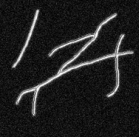
\includegraphics[height=1.5in]{benchImages/Synth-QuantitativeIFS-Fig7_gray.png}
        \caption{Red de filamentos sint\'etica disponible en \cite{qiu2014quantitative}.}
        \label{fig:synth-QFS-7-original}
    \end{subfigure}%
    \hspace{0.5cm}
    \begin{subfigure}[t]{0.3\textwidth}
        \centering
        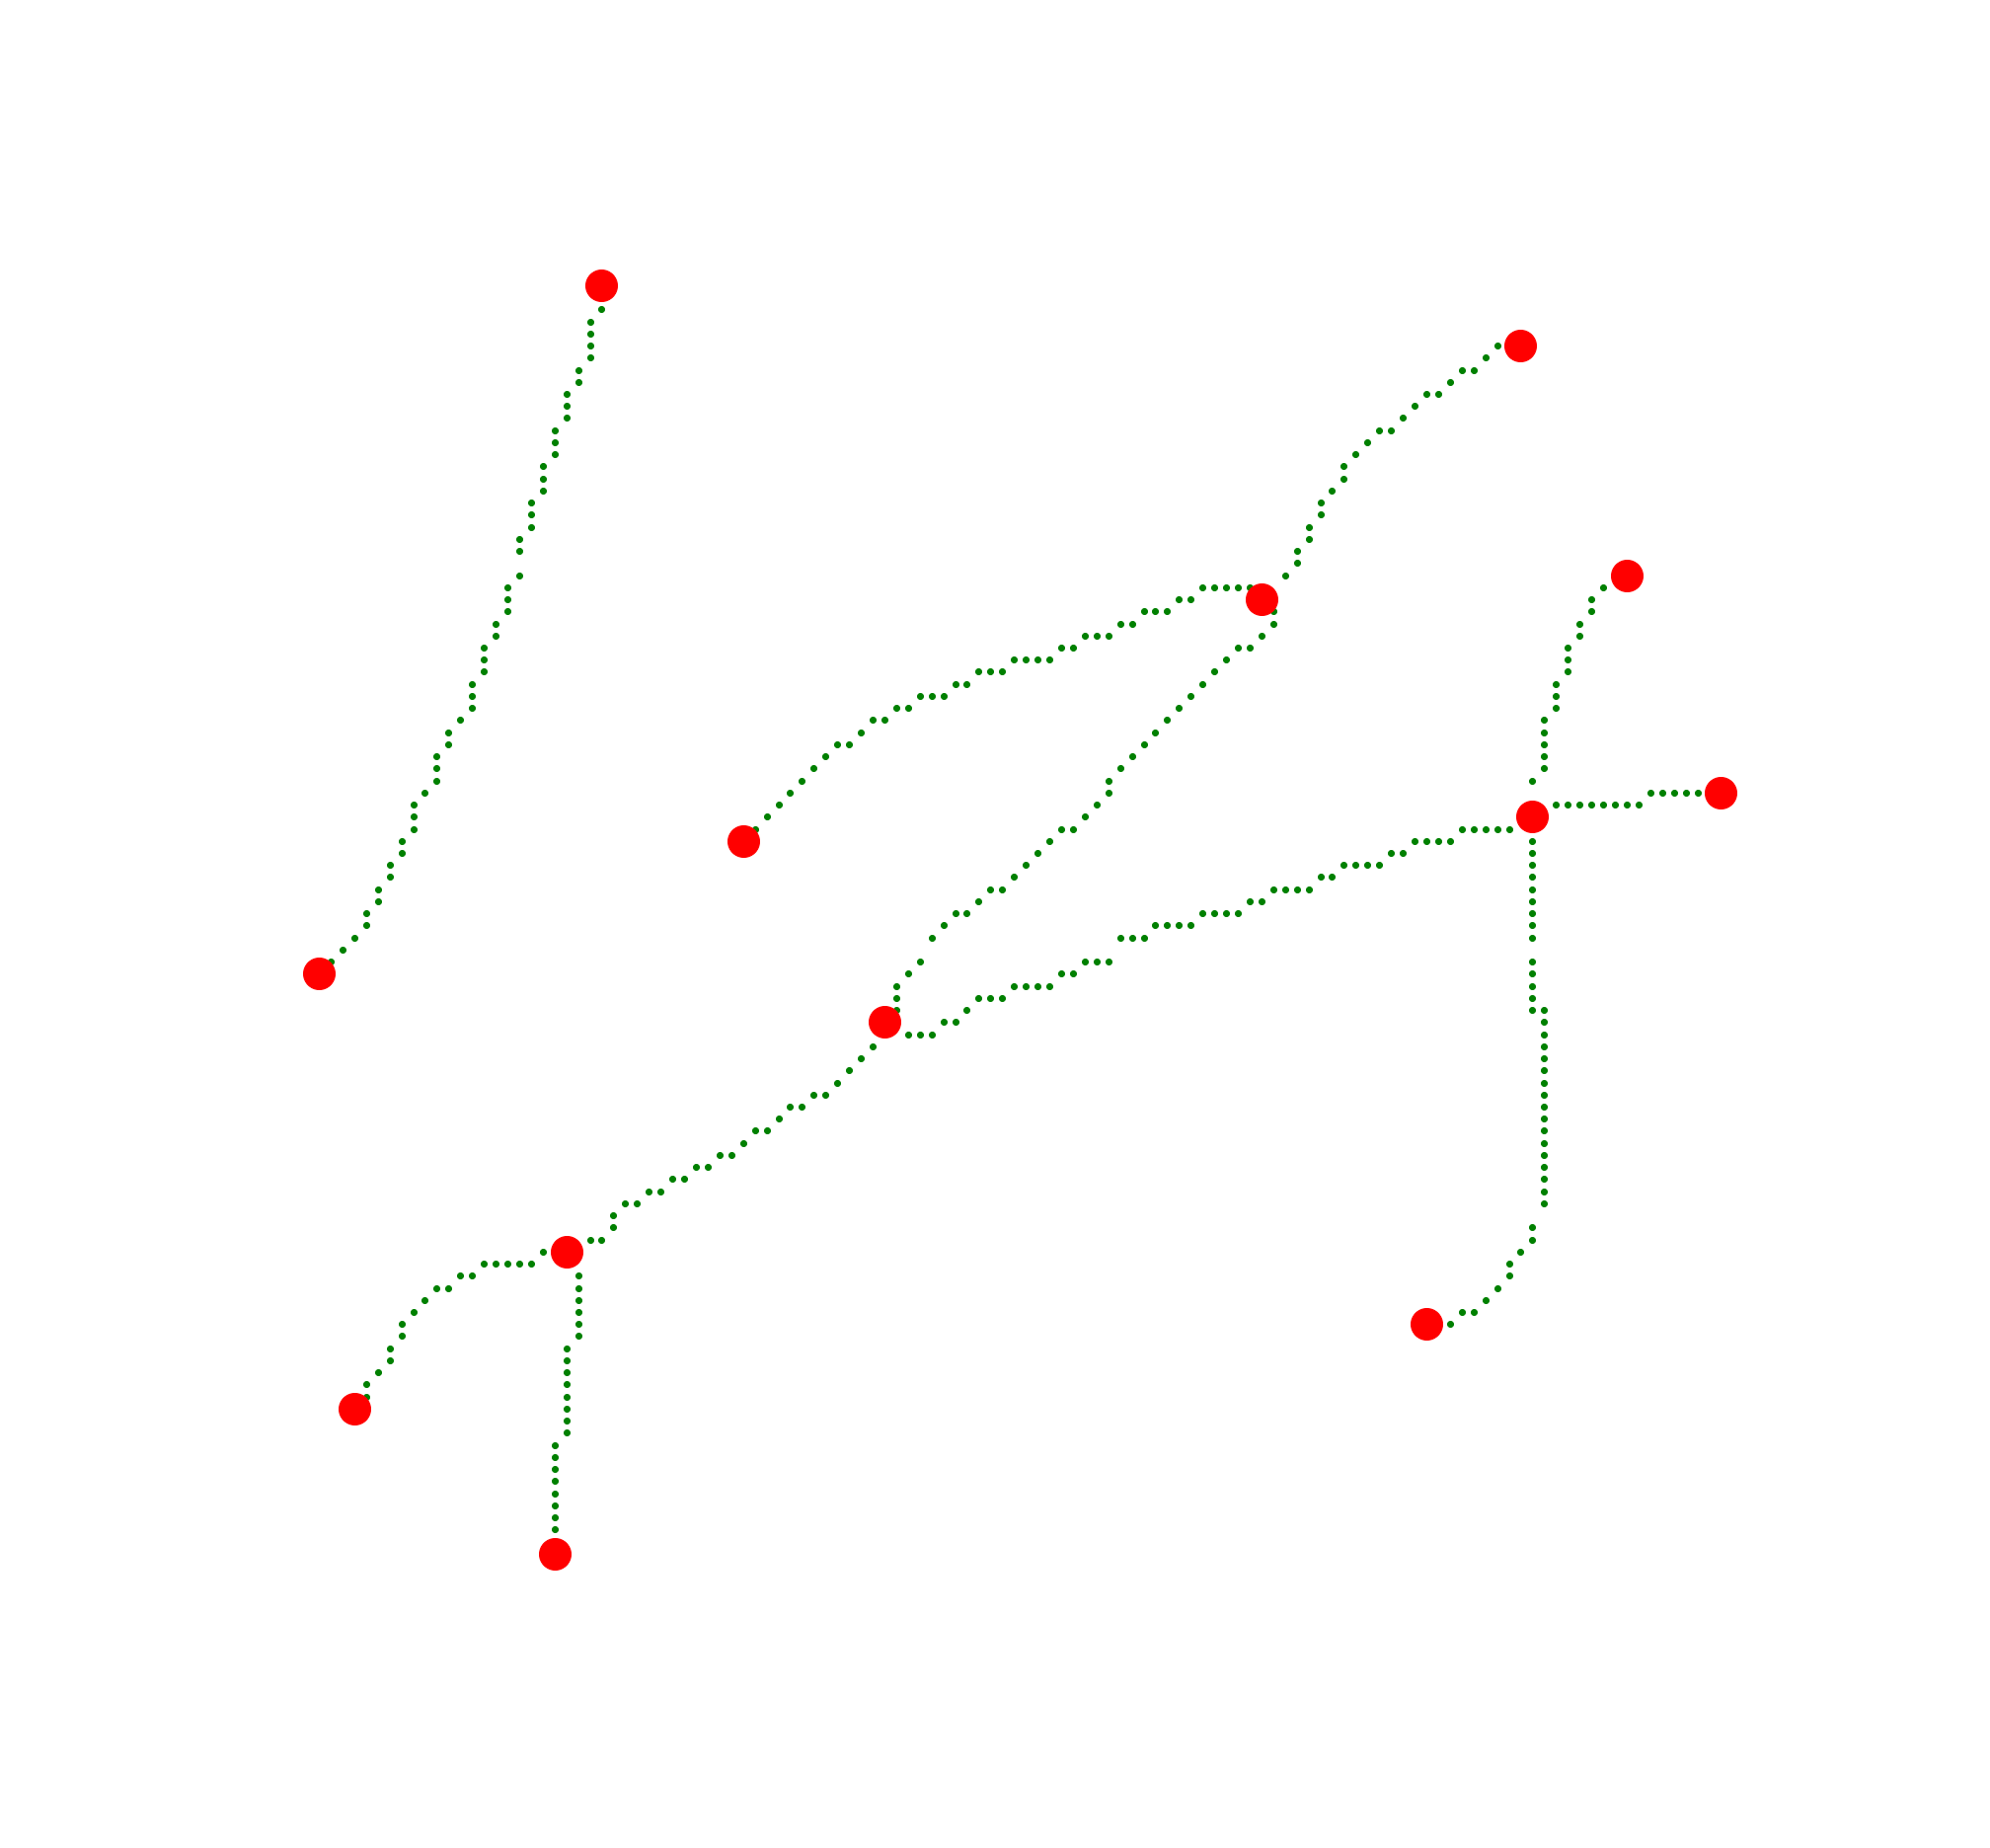
\includegraphics[height=1.5in]{benchImages/Synth-QuantitativeIFS-Fig7_graph_labeled_thick.png}
        \caption{Grafo extra\'ido de (a) utilizando la herramienta {\it sknw}.}
        \label{fig:synth-QFS-7-graph}
    \end{subfigure}
    \hspace{0.5cm}
    \begin{subfigure}[t]{0.3\textwidth}
        \centering
        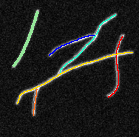
\includegraphics[height=1.5in]{benchImages/Synth-QuantitativeIFS-Fig7_groundTruth.png}
        \caption{Individualizaci\'on manual de (a).}
        \label{fig:synth-QFS-7-gt}
    \end{subfigure}
    \caption{Filamentos sint\'eticos. a) Los colores originales hacen referencia a la segmentaci\'on de filamentos en vez de la individualizaci\'on, por lo que se utiliza la imagen en escala de grises. b) Grafo de 11 aristas extra\'ido. c) Individualizaci\'n manual utilizando codificaci\'on por colores.}
    \label{fig:synth-QFS-7}
\end{figure*}


 \begin{figure*}[h!]
    \centering
    \begin{subfigure}[t]{0.3\textwidth}
        \centering
        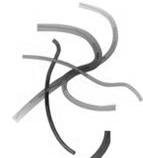
\includegraphics[height=1.5in]{benchImages/define-weighted-4.png}
        \caption{Red artificial de filamentos extra\'ida de una secci\'on de la Figura 1b en \cite{breuer2015define}.}
        \label{fig:synth-Define-1b-original}
    \end{subfigure}%
    \hspace{0.5cm}
    \begin{subfigure}[t]{0.3\textwidth}
        \centering
        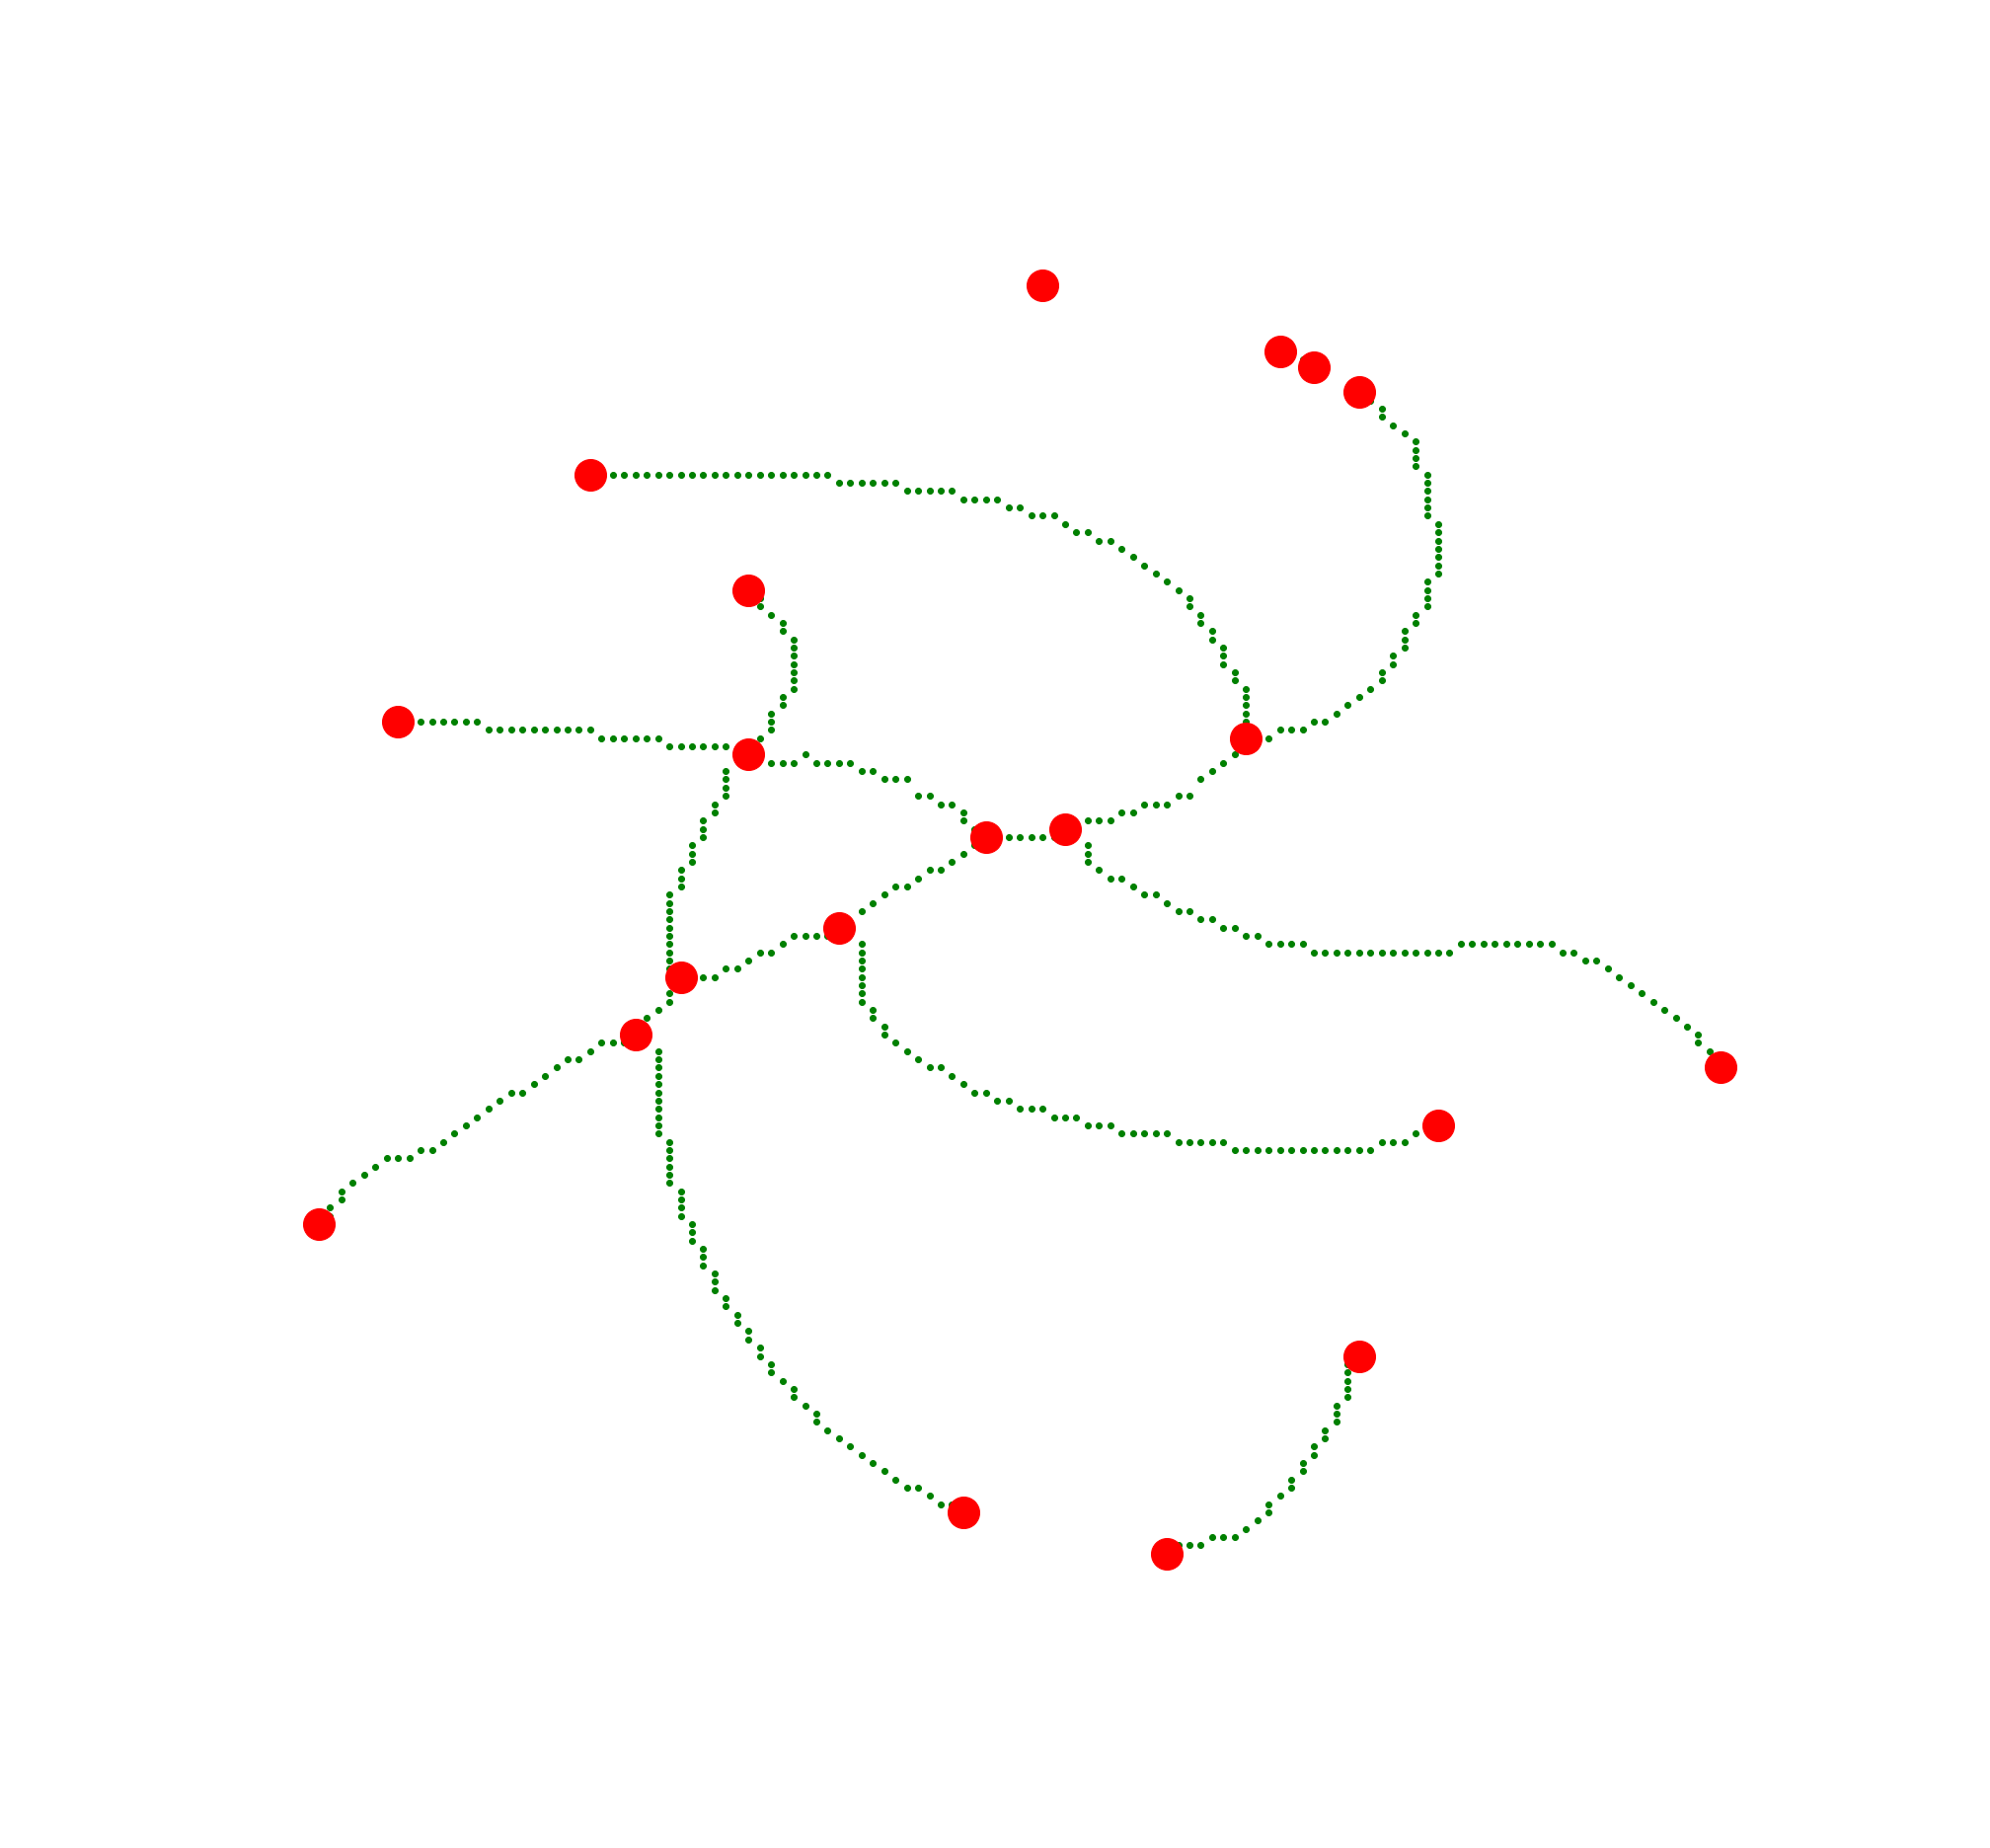
\includegraphics[height=1.5in]{benchImages/define-weighted-4_inv_graph_labeled_thick.png}
        \caption{Grafo extra\'ido de (a) utilizando {\it sknw}.}
        \label{fig:synth-Define-1b-graph}
    \end{subfigure}
    \hspace{0.5cm}
    \begin{subfigure}[t]{0.3\textwidth}
        \centering
        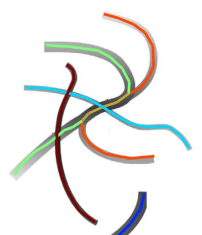
\includegraphics[height=1.5in]{benchImages/define-weighted-4-groundTruth.png}
        \caption{Individualizaci\'on manual de filamentos.}
        \label{fig:synth-Define-1b-graph-gt}
    \end{subfigure}
    \caption{Red sin\'etica de filamentos a) Secci\'on de la Figura 1b en \cite{breuer2015define}, correspondiente a una red sint\'etica de filamentos que abarca casos de sobreposici\'on y cruce. b) Grafo de 17 aristas. Se puede observar que el final de la arista superior derecha, o una discontinuidad que generando una arista y un nodo adicional. c) Codificaci\'on por colores para individualizar filamentos. La secci\'on de color cafe claro corresponde a un caso de superposici\'on entre dos filamentos.}
    \label{fig:synth-Define-1b}
\end{figure*}

Para la evaluaci\'on, cada imagen sint\'etica se ejecuta en DeFiNe con los par\'ametros base {\tt BFS - Overlapping - Pairwise - Total}, ya que fueron los de mejor resultado en \cite{breuer2015define}, configurando el \'angulo de umbral en 30\textdegree y 60\textdegree. Por su parte, el algoritmo propuesto se ejecuta 5 veces con distintas semillas.

\section{Im\'agenes Reales}
%1.- pasos para la obtenci\'on de los filamentos desde las imagenes
% 2.- extraccion del grafo mediante skeletonizacion usando sknw que deja el grafo en networkX. Necesidad de una imagen con fondo negro y binaria
%3.- paso del grafo a gml para comparar con define
%4.-paso del grafo a json para integrar a algoritmo propuesto
El procedimiento para individualizar filamentos en im\'agenes de microscop\'ia
comienza de forma similar para las c\'elulas observadas en esta investigaci\'on, consistiendo en el an\'alisis del {\it stack} o conjunto de im\'agenes capturadas durante una observaci\'on, las que pueden variar en el tiempo y en el eje Z. El criterio principal utilizado por los expertos se basa en determinar si existe continuidad de un posible filamento entre dos o m\'as im\'agenes del stack. %Adem\'as, el experto busca descartar la influencia de ruido en la continuidad que pueden generar 

Al observar un {\it stack}, el experto anota los filamentos de la c\'elula mediante la selecci\'on del \'area de inter\'es o ROI sobre una imagen que proyecta la uni\'on de las im\'agenes del stack bajo alg\'un criterio asociado a la intensidad de los p\'ixeles en el eje Z. Las Figuras \ref{fig:SpinningMarchantia-gt}, \ref{fig:field3t0filtered1-gt} y \ref{fig:field3t0filtered2-gt} son ejemplos de las anotaciones de ROIs para microt\'ubulos realizadas. A diferencia de las neuronas, donde se procesa la imagen completa, la elecci\'on de un subconjunto de microt\'ubulos desde la imagen se debe a la complejidad de la individualizaci\'on manual de estos por parte del experto. Se diferenciaran las im\'agenes de microt\'ubulos de las Figuras \ref{fig:SpinningMarchantia}, \ref{fig:field3t0filtered1} y \ref{fig:field3t0filtered2} bajo la denominaci\'on de muestra MT-A, MT-B y MT-C respectivamente. Por su parte, las im\'agenes de neuronas de las Figuras \ref{fig:Porta6-4a1}, \ref{fig:Porta10-5b} y \ref{fig:Porta18-3a1}  se denominan N1, N2 y N3 respectivamente.

Una vez obtenida la individualizaci\'on manual de filamentos, independientemente del tipo de c\'elula, se construye una segmentaci\'on de las \'areas de inter\'es con el fin de generar una codificaci\'on de colores del {\it ground truth}, generandose tambi\'en el grafo que representa la red de filamentos. La codificaci\'on de colores permite una comparaci\'on visual con los resultados de DeFiNe o de el algoritmo propuesto. Por su parte, el grafo se obtiene mediante la extracci\'on de un esqueleto desde la imagen segmentada al utilizar la herramienta {\it sknw}, parte del software {\it ImagePy}\cite{wang2018imagepy}. A partir del grafo se calcula el {\it closeness centrality}\cite{freeman1978centrality}, que mide la lejan\'ia promedio de cada nodo con respecto al resto, otorgando un valor m\'as alto a los nodos que se encuentran m\'as cerca de todos los dem\'as. La selecci\'on de los 3 nodos de mayor valor proporciona informaci\'on de la ubicaci\'on del {\tt soma} en el caso de las neuronas.


Posteriormente, el grafo es escrito a un archivo en los formatos GML y JSON, los que son utilizados como archivos de entrada en DeFiNe y en ael lgoritmo propuesto respectivamente, para la individualizaci\'on autom\'atica de filamentos.
Las resultados de cada imagen analizada en el algoritmo propuesto se obtienen con el mismo procedimiento utilizado para las im\'agenes sint\'eticas.
%la cual requiere que la imagen de proyecci\'on del eje Z se encuentre en modo binario con el fondo negro. Finalmente a partir del grafo, es posible obtener un archivo en formato GML y otro en formato JSON, 


%Spinning
\begin{figure*}[h!]
    \centering
    \begin{subfigure}[t]{0.49\textwidth}
        \centering
        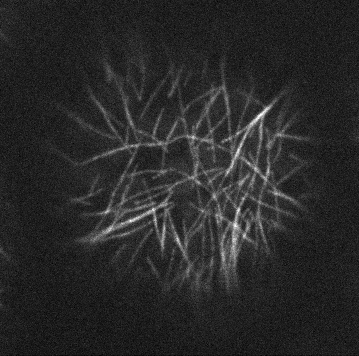
\includegraphics[height=2.2in]{benchImages/AVG-SPINNING-DISK-MARCHANTIA.png}
        \caption{Imagen de Microt\'ubulos.}
        \label{fig:SpinningMarchantia-og}
    \end{subfigure}
    ~ 
    \begin{subfigure}[t]{0.49\textwidth}
        \centering
        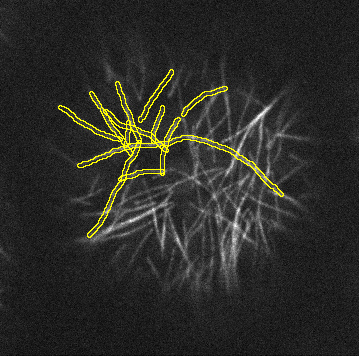
\includegraphics[height=2.2in]{benchImages/SPINNING-DISK-MARCHANTIA-rois-unlabeled.png}
        \caption{Filamentos manualmente individualizados por un experto.}
        \label{fig:SpinningMarchantia-gt}
    \end{subfigure}
    \vskip\baselineskip
    \begin{subfigure}[t]{0.49\textwidth}
        \centering
        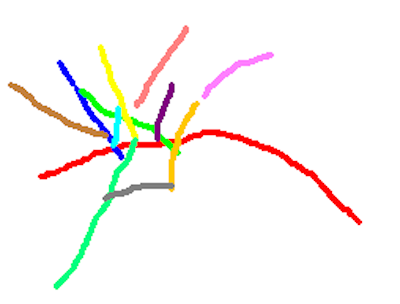
\includegraphics[height=2.2in]{benchImages/50-ROIs-Spinning-Marchantia-solved-rot-unlabeled.png}
        \caption{Codificaci\'on por color de la individualizaci\'on manual.}
        \label{fig:SpinningMarchantia-indivManual}
    \end{subfigure}
    ~
    \begin{subfigure}[t]{0.49\textwidth}
        \centering
        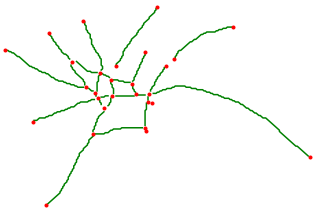
\includegraphics[height=2.2in]{benchImages/50-ROIs-Spinning-Marchantia-graph-og.png}
        \caption{Grafo que representa la red de microt\'ubulos manualmente identificada.}
        \label{fig:SpinningMarchantia-graph}
    \end{subfigure}
    \caption{Individualizaci\'on manual de microt\'ubulos. a) Imagen 6 de un stack de 301 cuadros de {\it Arabidopsis Marchantia}. b) Individualizaci\'on manual c) Representaci\'on mediante colores de los diferentes microt\'ubulos. d) Grafo de 29 aristas extra\'ido a partir de la individualizaci\'on manual, que es el dato de entrada para los algoritmos comparados.}
    \label{fig:SpinningMarchantia}
\end{figure*}



%field3t02Bcell-filtered1
\begin{figure*}[h!]
    \centering
    \begin{subfigure}[t]{0.49\textwidth}
        \centering
        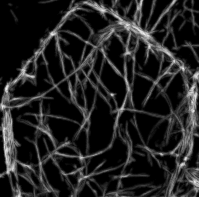
\includegraphics[height=2.2in]{benchImages/field3-t0-2cellBcrop-filtered-1.png}
        \caption{Imagen de Microt\'ubulos.}
        \label{fig:field3t0filtered1-og}
    \end{subfigure}
    ~ 
    \begin{subfigure}[t]{0.49\textwidth}
        \centering
        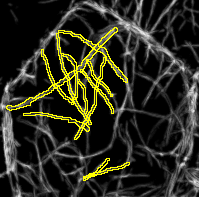
\includegraphics[height=2.2in]{benchImages/field3-t0-2cellBcrop-filtered-1-rois.png}
        \caption{Filamentos manualmente individualizados por un experto.}
        \label{fig:field3t0filtered1-gt}
    \end{subfigure}
    \vskip\baselineskip
    \begin{subfigure}[t]{0.49\textwidth}
        \centering
        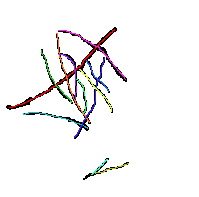
\includegraphics[height=2.2in]{benchImages/field3-t0-2cellBcrop-filtered-inverted-colorCoded.png}
        \caption{Codificaci\'on por color de la individualizaci\'on manual.}
        \label{fig:field3t0filtered1-indivManual}
    \end{subfigure}
    ~
    \begin{subfigure}[t]{0.49\textwidth}
        \centering
        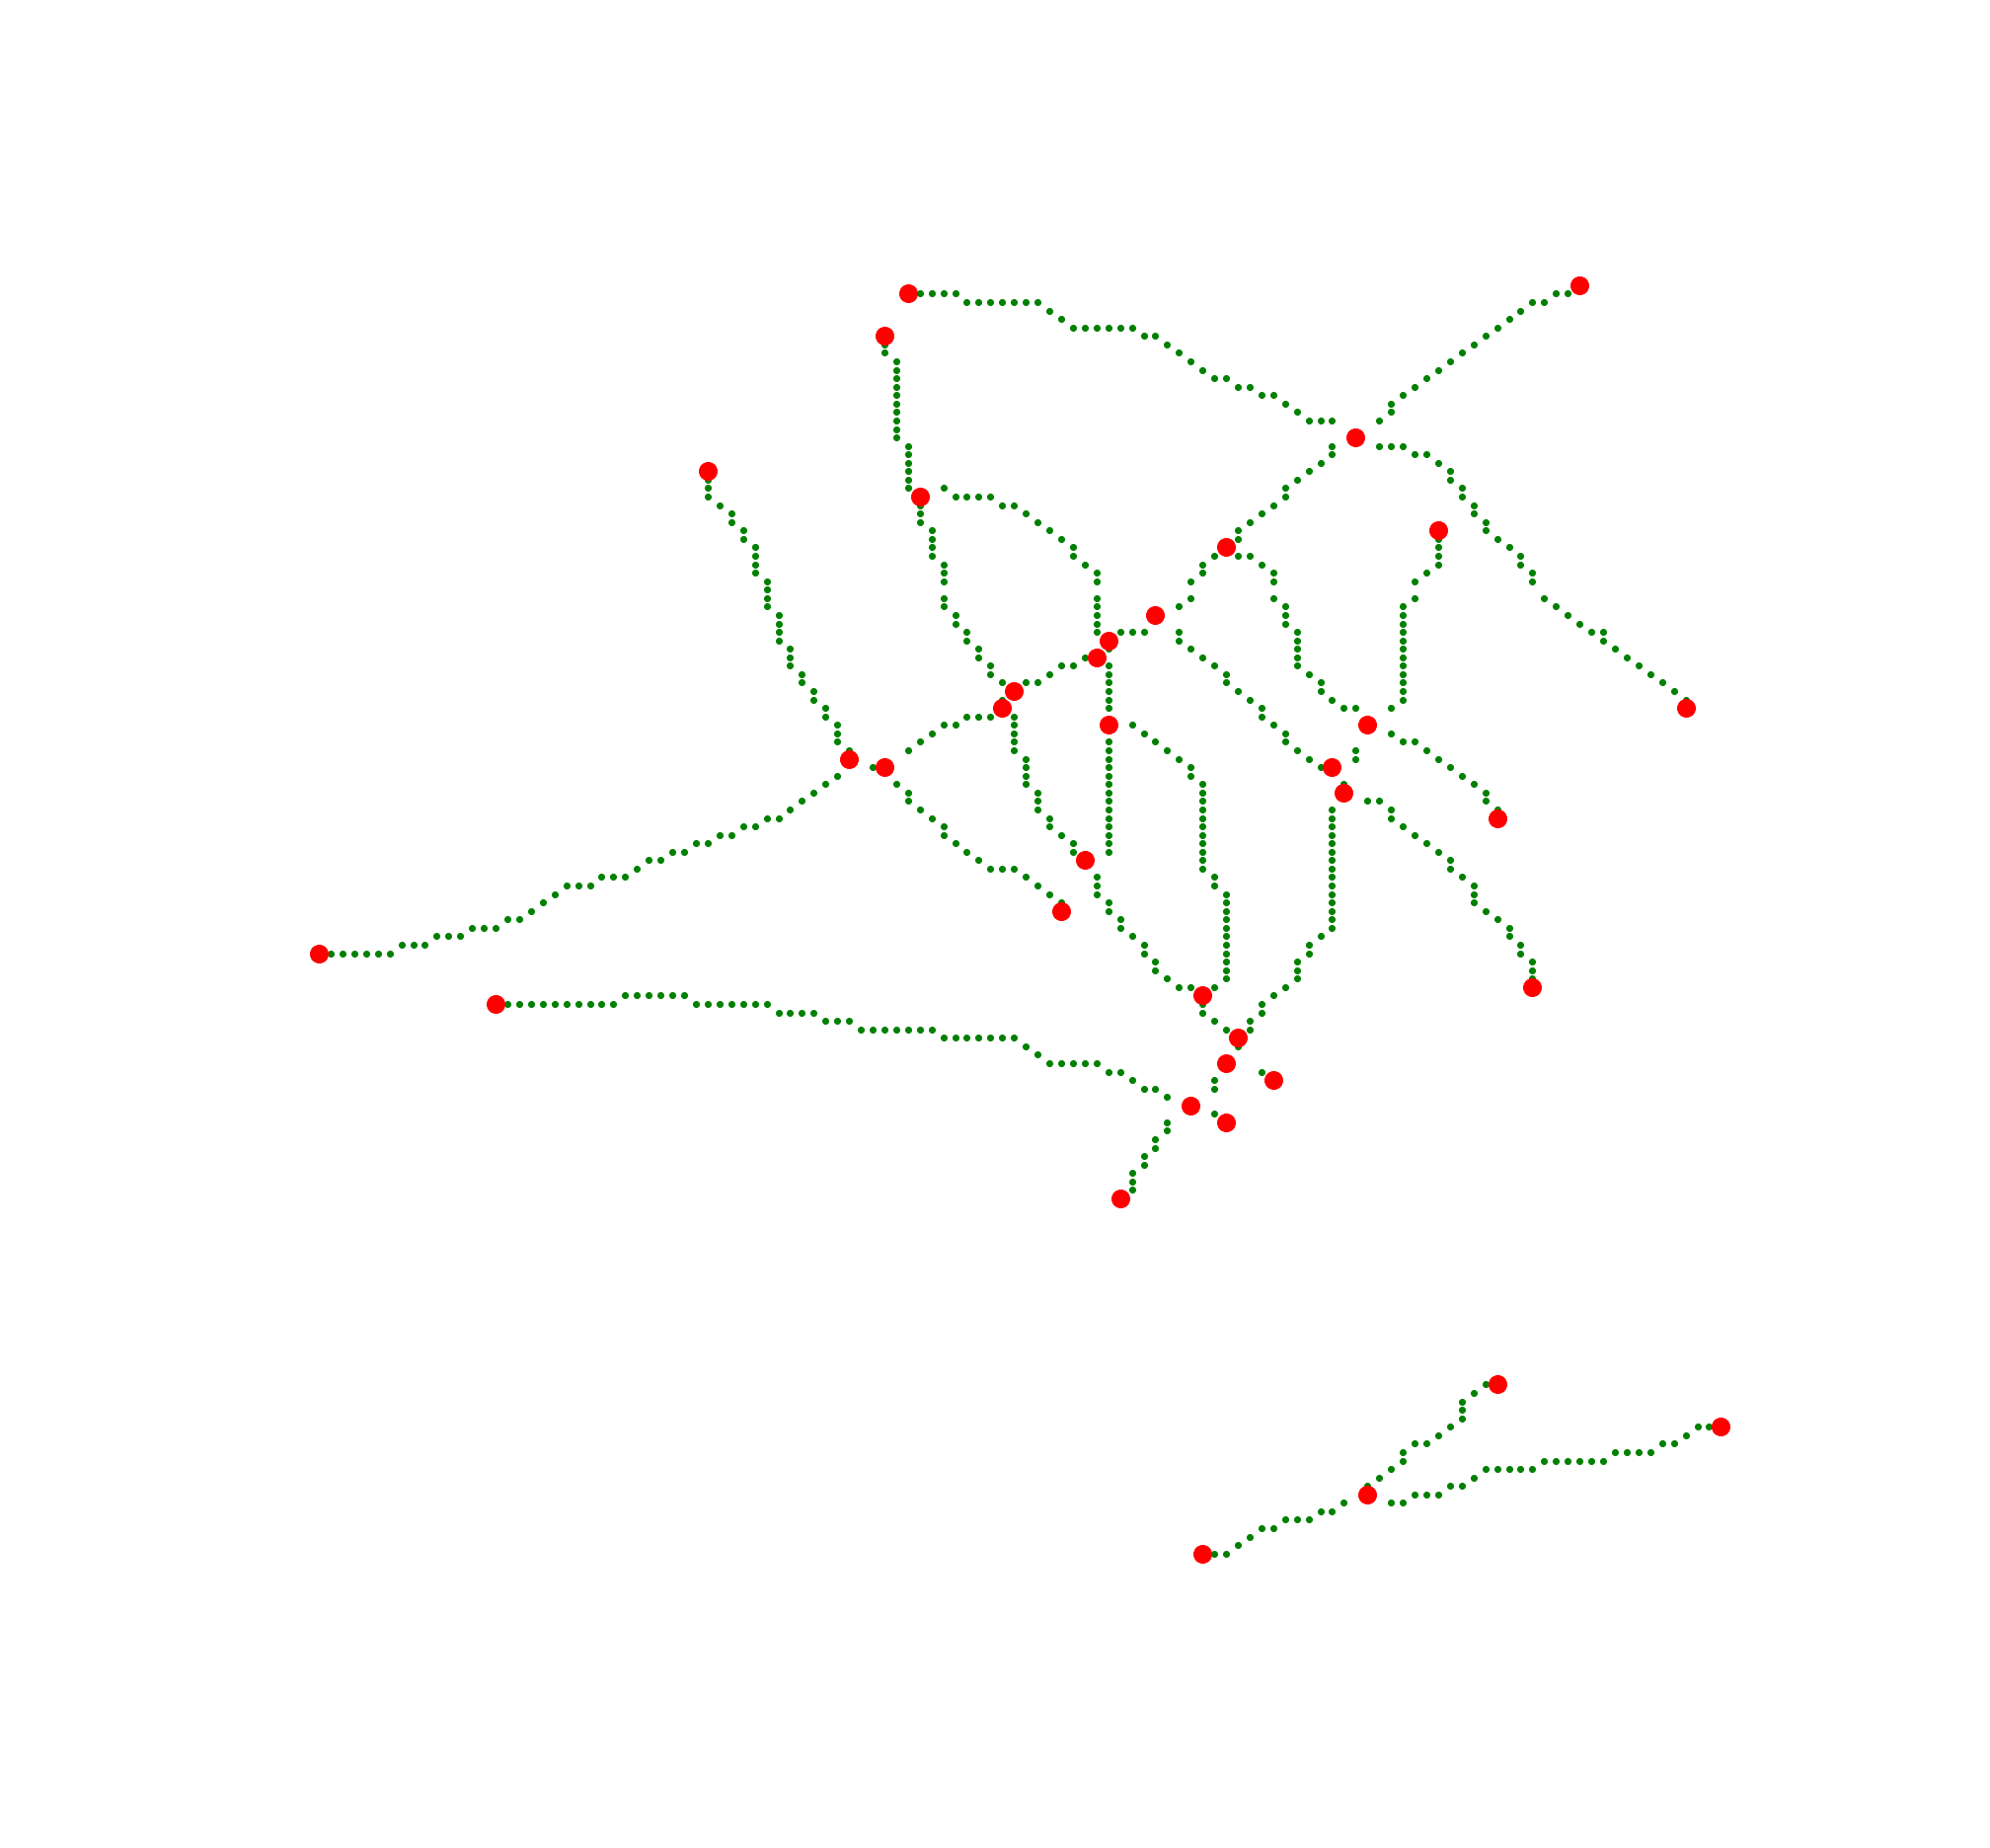
\includegraphics[height=2.2in]{benchImages/field3-t0-2cellBcrop-filtered-graph-thick.png}
        \caption{Grafo extra\'ido a partir de la individualizaci\'on manual que es el dato de entrada para los algoritmos comparados.}
        \label{fig:field3t0filtered1-graph}
    \end{subfigure}
    \caption{Individualizaci\'on manual de microt\'ubulos. a) Imagen de {\it Arabidopsis Marchantia} obtenida al realizar la proyecci\'on del eje Z bajo el criterio de promedio de p\'ixeles. b) \'Areas de inter\'es de la individualizaci\'on manual c) Representaci\'on mediante colores de los diferentes microt\'ubulos. d) Grafo de 40 aristas utilizado en la individualizaci\'on autom\'atica de filamentos.}
    \label{fig:field3t0filtered1}
\end{figure*}



%field3t02Bcell-filtered2
\begin{figure*}[h!]
    \centering
    \begin{subfigure}[t]{0.49\textwidth}
        \centering
        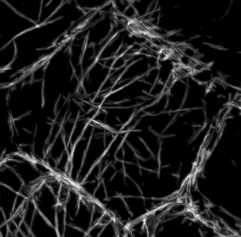
\includegraphics[height=2.2in]{benchImages/field3-t0-2cellBcrop-filtered-2.png}
        \caption{Imagen de Microt\'ubulos.}
        \label{fig:field3t0filtered2-og}
    \end{subfigure}
    ~ 
    \begin{subfigure}[t]{0.49\textwidth}
        \centering
        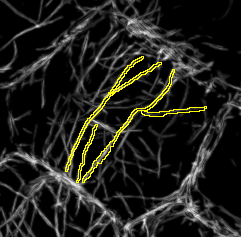
\includegraphics[height=2.2in]{benchImages/field3-t0-2cellBcrop-filtered-2-rois.png}
        \caption{Filamentos manualmente individualizados por un experto.}
        \label{fig:field3t0filtered2-gt}
    \end{subfigure}
    \vskip\baselineskip
    \begin{subfigure}[t]{0.49\textwidth}
        \centering
        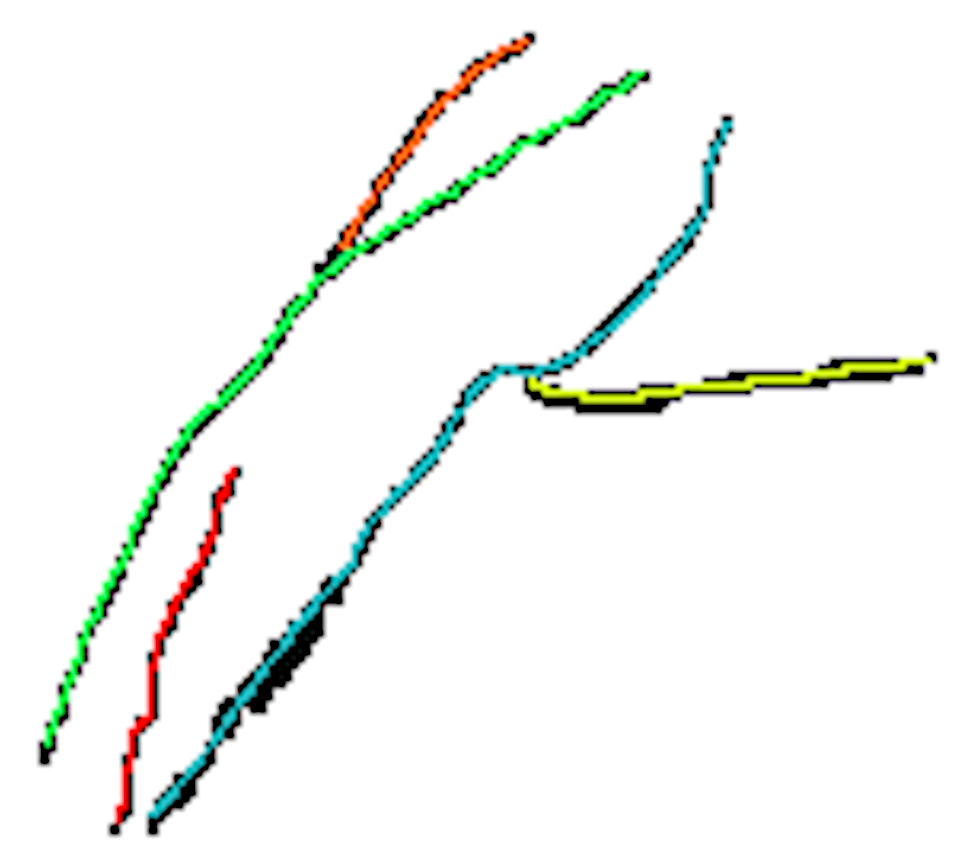
\includegraphics[height=2.2in]{benchImages/field3-t0-2cellBcrop-filtered-2-inverted-colorCoded.png}
        \caption{Codificaci\'on por color de la individualizaci\'on manual.}
        \label{fig:field3t0filtered2-indivManual}
    \end{subfigure}
    ~
    \begin{subfigure}[t]{0.49\textwidth}
        \centering
        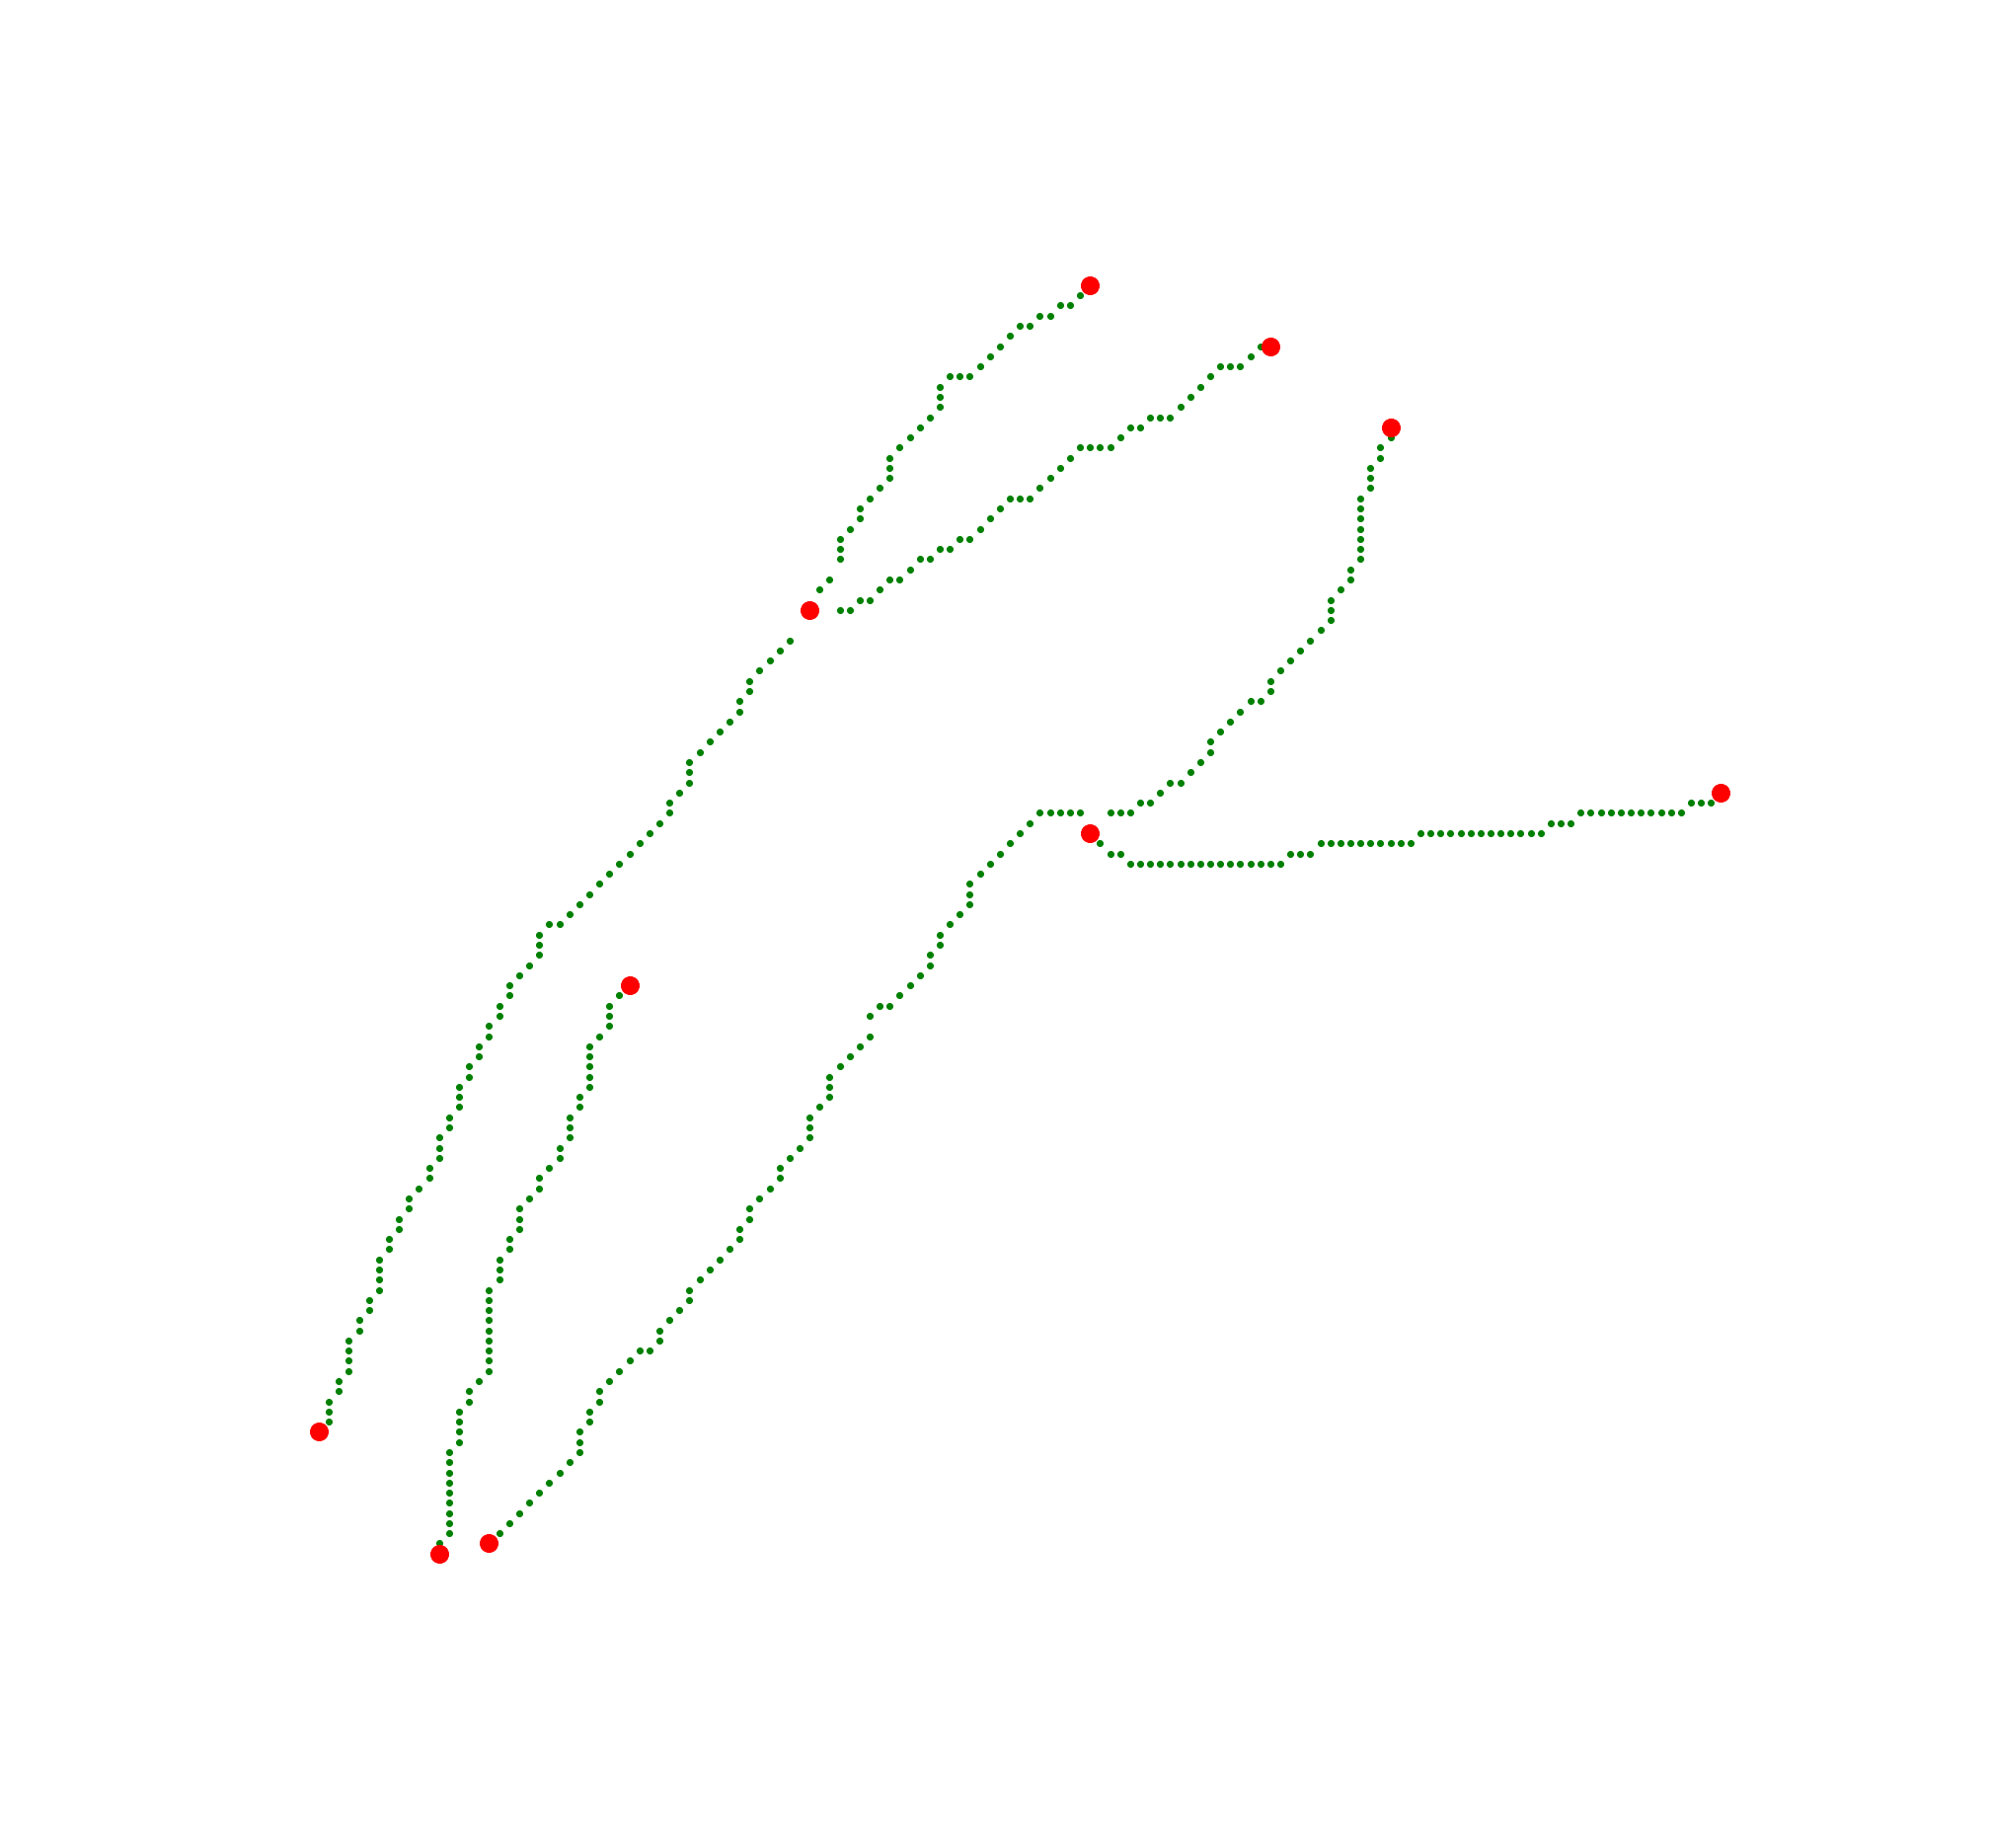
\includegraphics[height=2.2in]{benchImages/field3-t0-2cellBcrop-filtered-2-graph-thick.png}
        \caption{Grafo base para la individualizaci\'on automatizada de filamentos.}
        \label{fig:field3t0filtered2-graph}
    \end{subfigure}
    \caption{Individualizaci\'on manual de microt\'ubulos. a) Imagen de {\it Arabidopsis Marchantia} obtenida al realizar la proyecci\'on del eje Z bajo el criterio de promedio de p\'ixeles. b) \'Areas de inter\'es de la individualizaci\'on manual c) Representaci\'on mediante colores de los diferentes microt\'ubulos. d) Grafo de 7 aristas extra\'ido a partir de la individualizaci\'on manual.}
    \label{fig:field3t0filtered2}
\end{figure*}

%Porta6-4a1
\begin{figure*}[h!]
    \centering
    \begin{subfigure}[t]{0.49\textwidth}
        \centering
        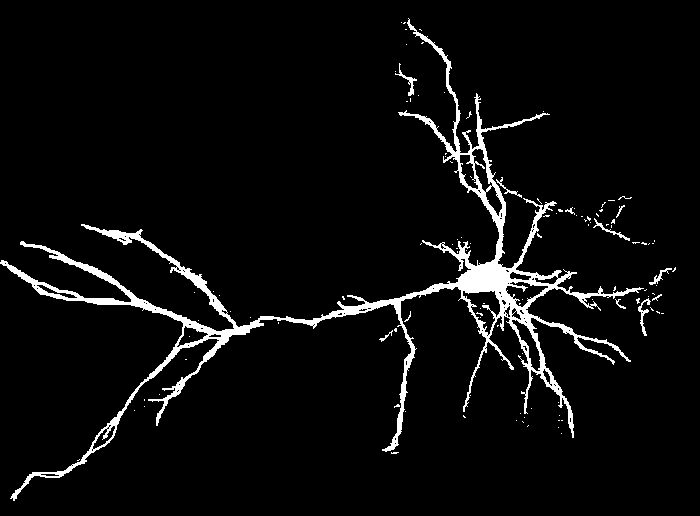
\includegraphics[height=2.2in]{benchImages/grupo3-Porta6-4a1-MAX-cleaned.png}
        \caption{Imagen de una neurona.}
        \label{fig:Porta6-4a1-og}
    \end{subfigure}
    ~ 
    \begin{subfigure}[t]{0.49\textwidth}
        \centering
        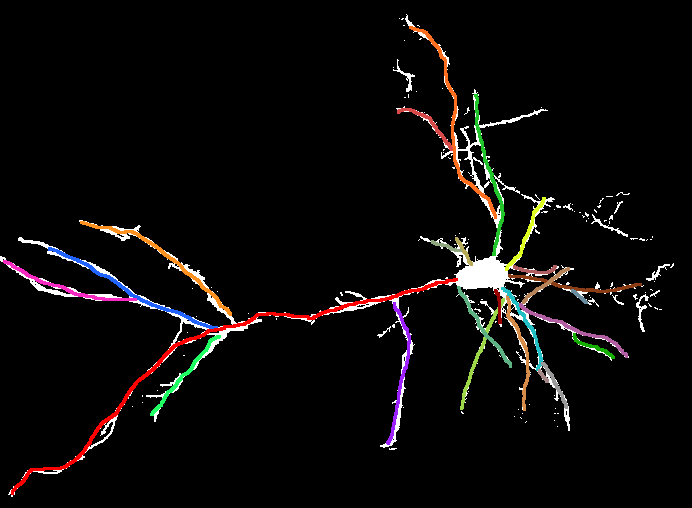
\includegraphics[height=2.2in]{benchImages/grupo3-Porta6-4a1-MAX-cleaned-colorCoded.png}
        \caption{Filamentos manualmente individualizados por un experto.}
        \label{fig:Porta6-4a1-gt}
    \end{subfigure}
\vskip\baselineskip
    \begin{subfigure}[t]{0.5\textwidth}
        \centering
        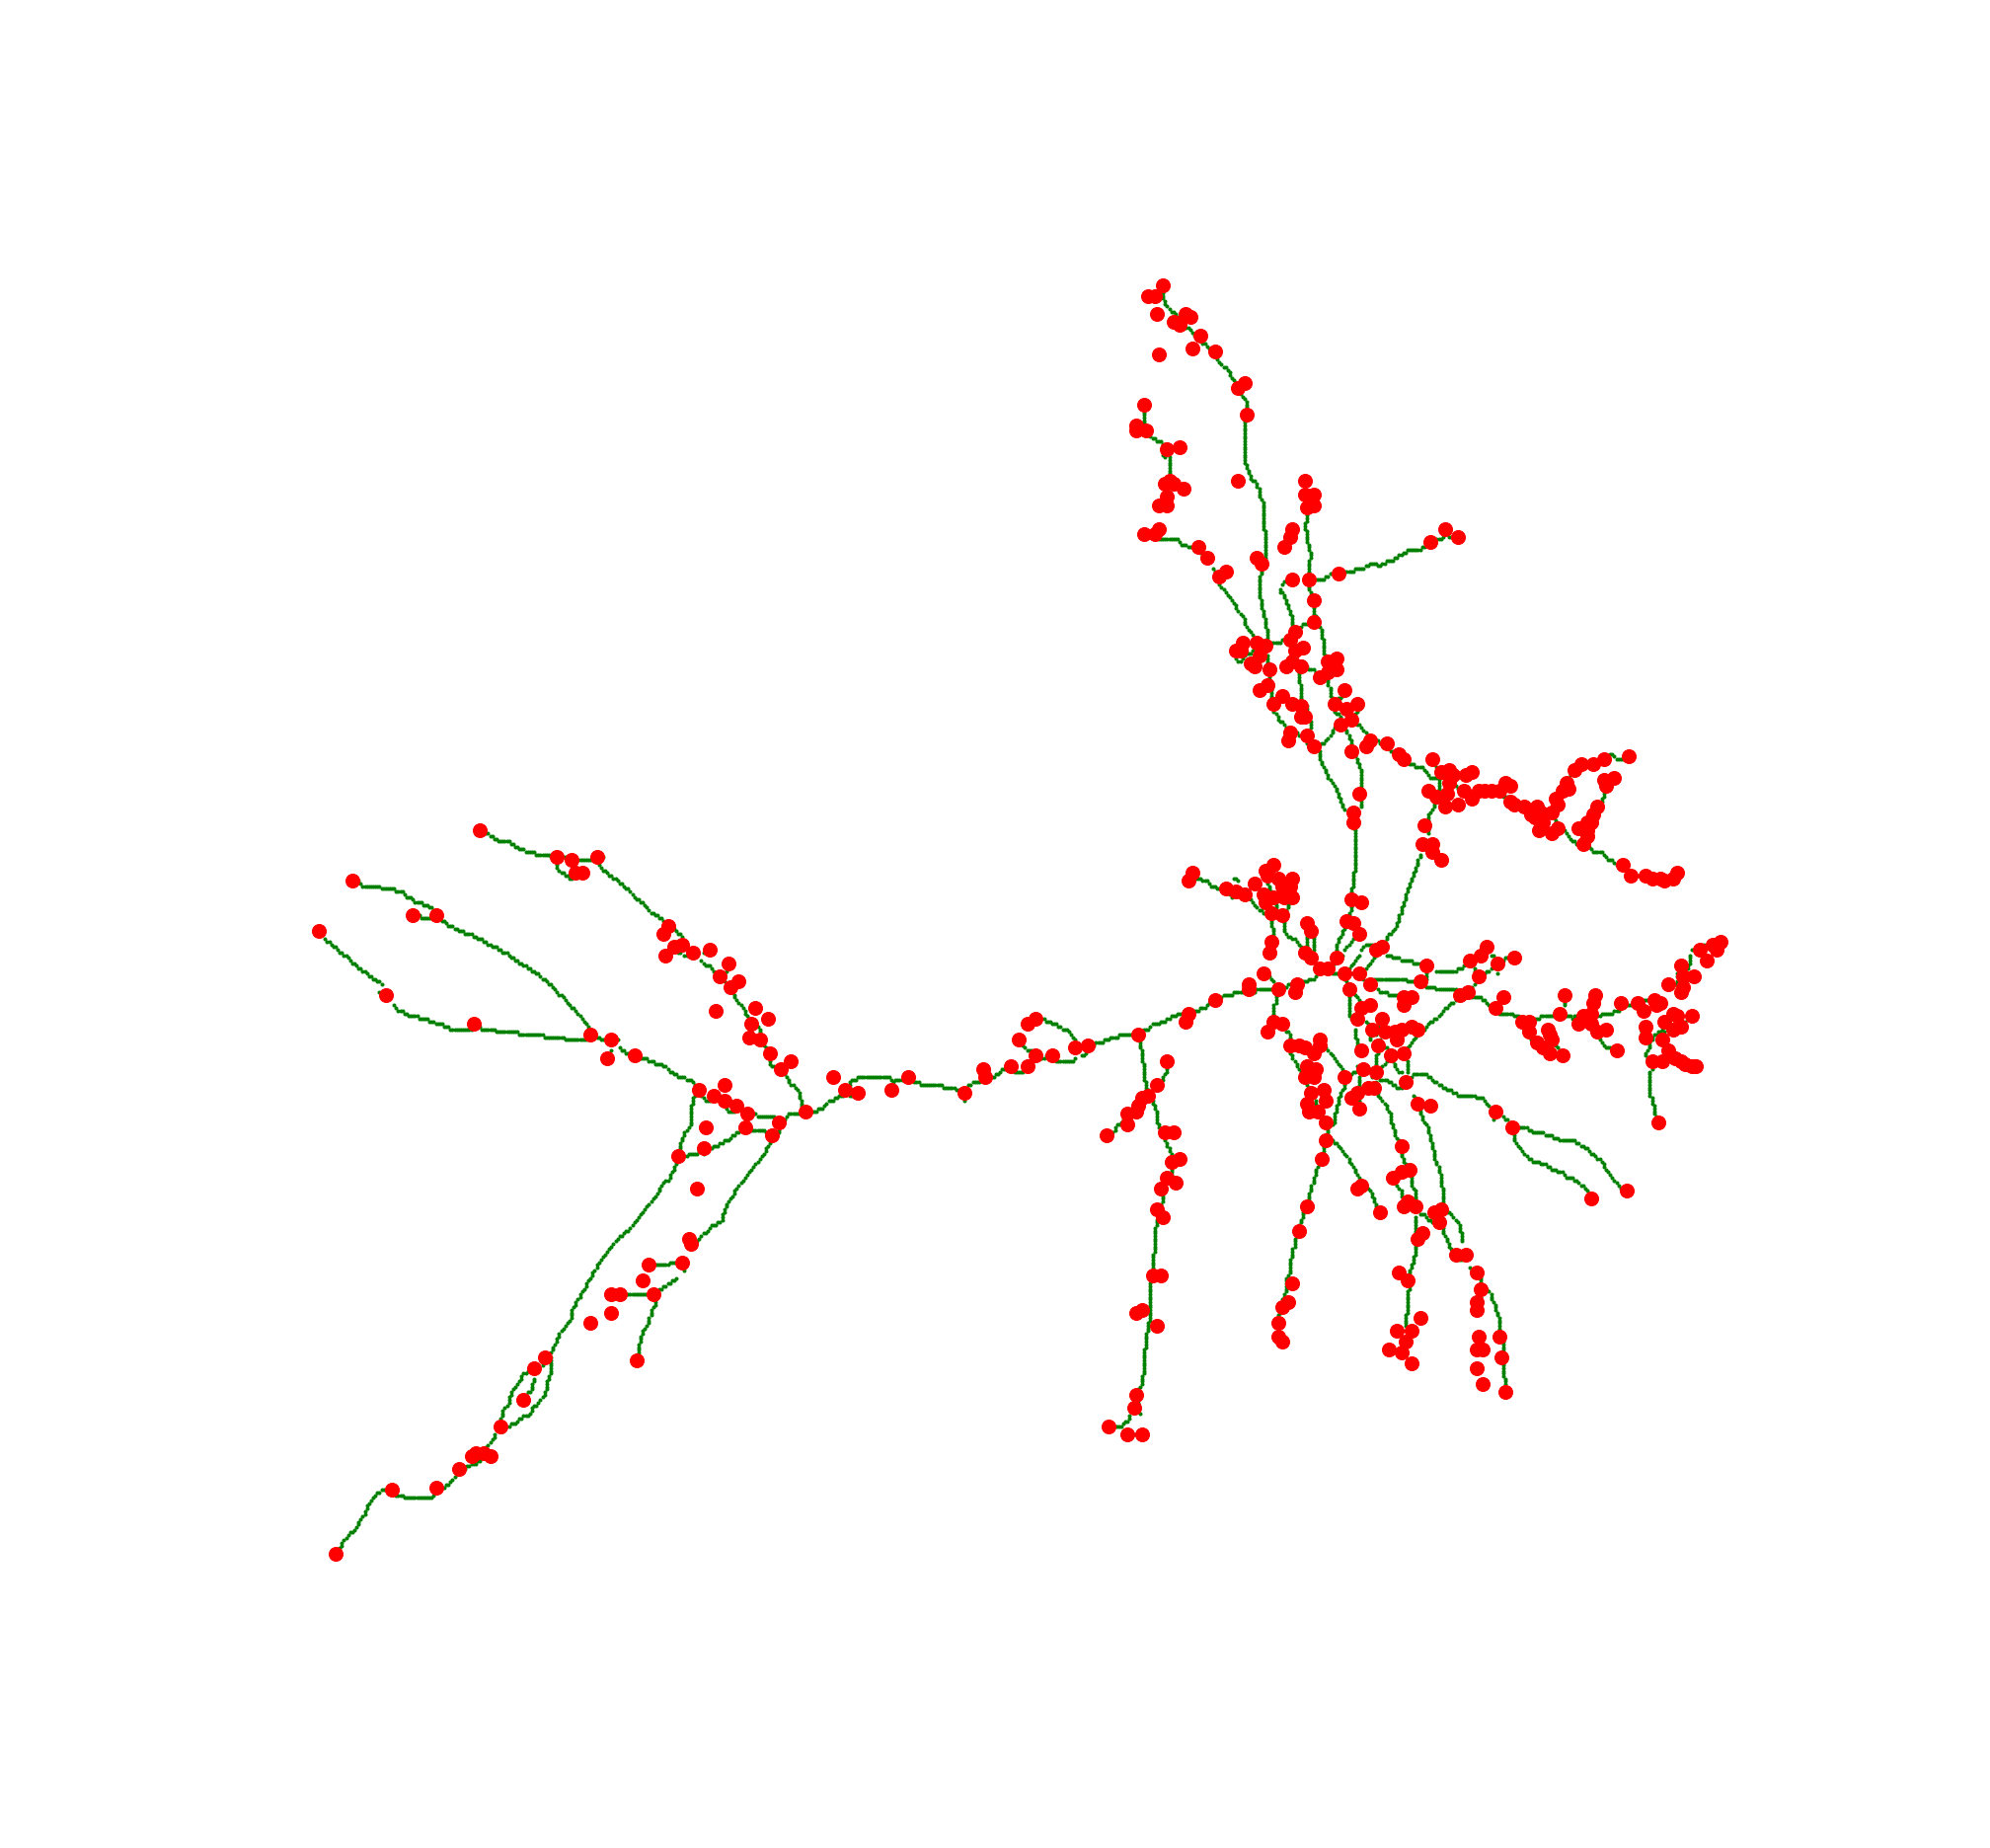
\includegraphics[height=2in]{benchImages/grupo3-Porta6-4a1-MAX-cleaned-graph-thick.png}
        \caption{Grafo base para la individualizaci\'on automatizada de filamentos.}
        \label{fig:Porta6-4a1-graph}
    \end{subfigure}
    \caption{Individualizaci\'on manual de una neurona. a) Imagen de ... obtenida al realizar la proyecci\'on del eje Z bajo el criterio de valor m\'aximo de p\'ixeles. b) Representaci\'on mediante colores de los filamentos de la neurona, representando el ax\'on y las dendritas. d) Grafo de X aristas extra\'ido a partir de la individualizaci\'on manual.}
    \label{fig:Porta6-4a1}
\end{figure*}

%Porta10-5b
\begin{figure*}[h!]
    \centering
    \begin{subfigure}[t]{0.49\textwidth}
        \centering
        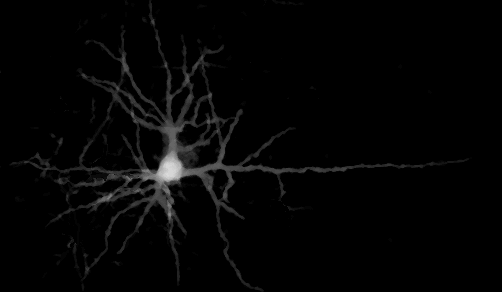
\includegraphics[height=1.9in]{benchImages/grupo1-Porta10-5b-AVG-partialCleaned.png}
        \caption{Imagen de una neurona.}
        \label{fig:Porta10-5b-og}
    \end{subfigure}
    ~ 
    \begin{subfigure}[t]{0.49\textwidth}
        \centering
        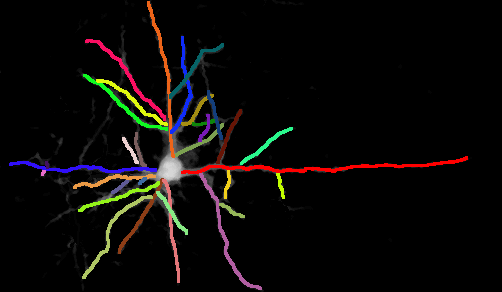
\includegraphics[height=1.9in]{benchImages/grupo1-Porta10-5b-AVG-partialCleaned-colorCoded.png}
        \caption{Filamentos manualmente individualizados por un experto.}
        \label{fig:Porta10-5b-gt}
    \end{subfigure}
    \vskip\baselineskip
    \begin{subfigure}[t]{0.5\textwidth}
        \centering
        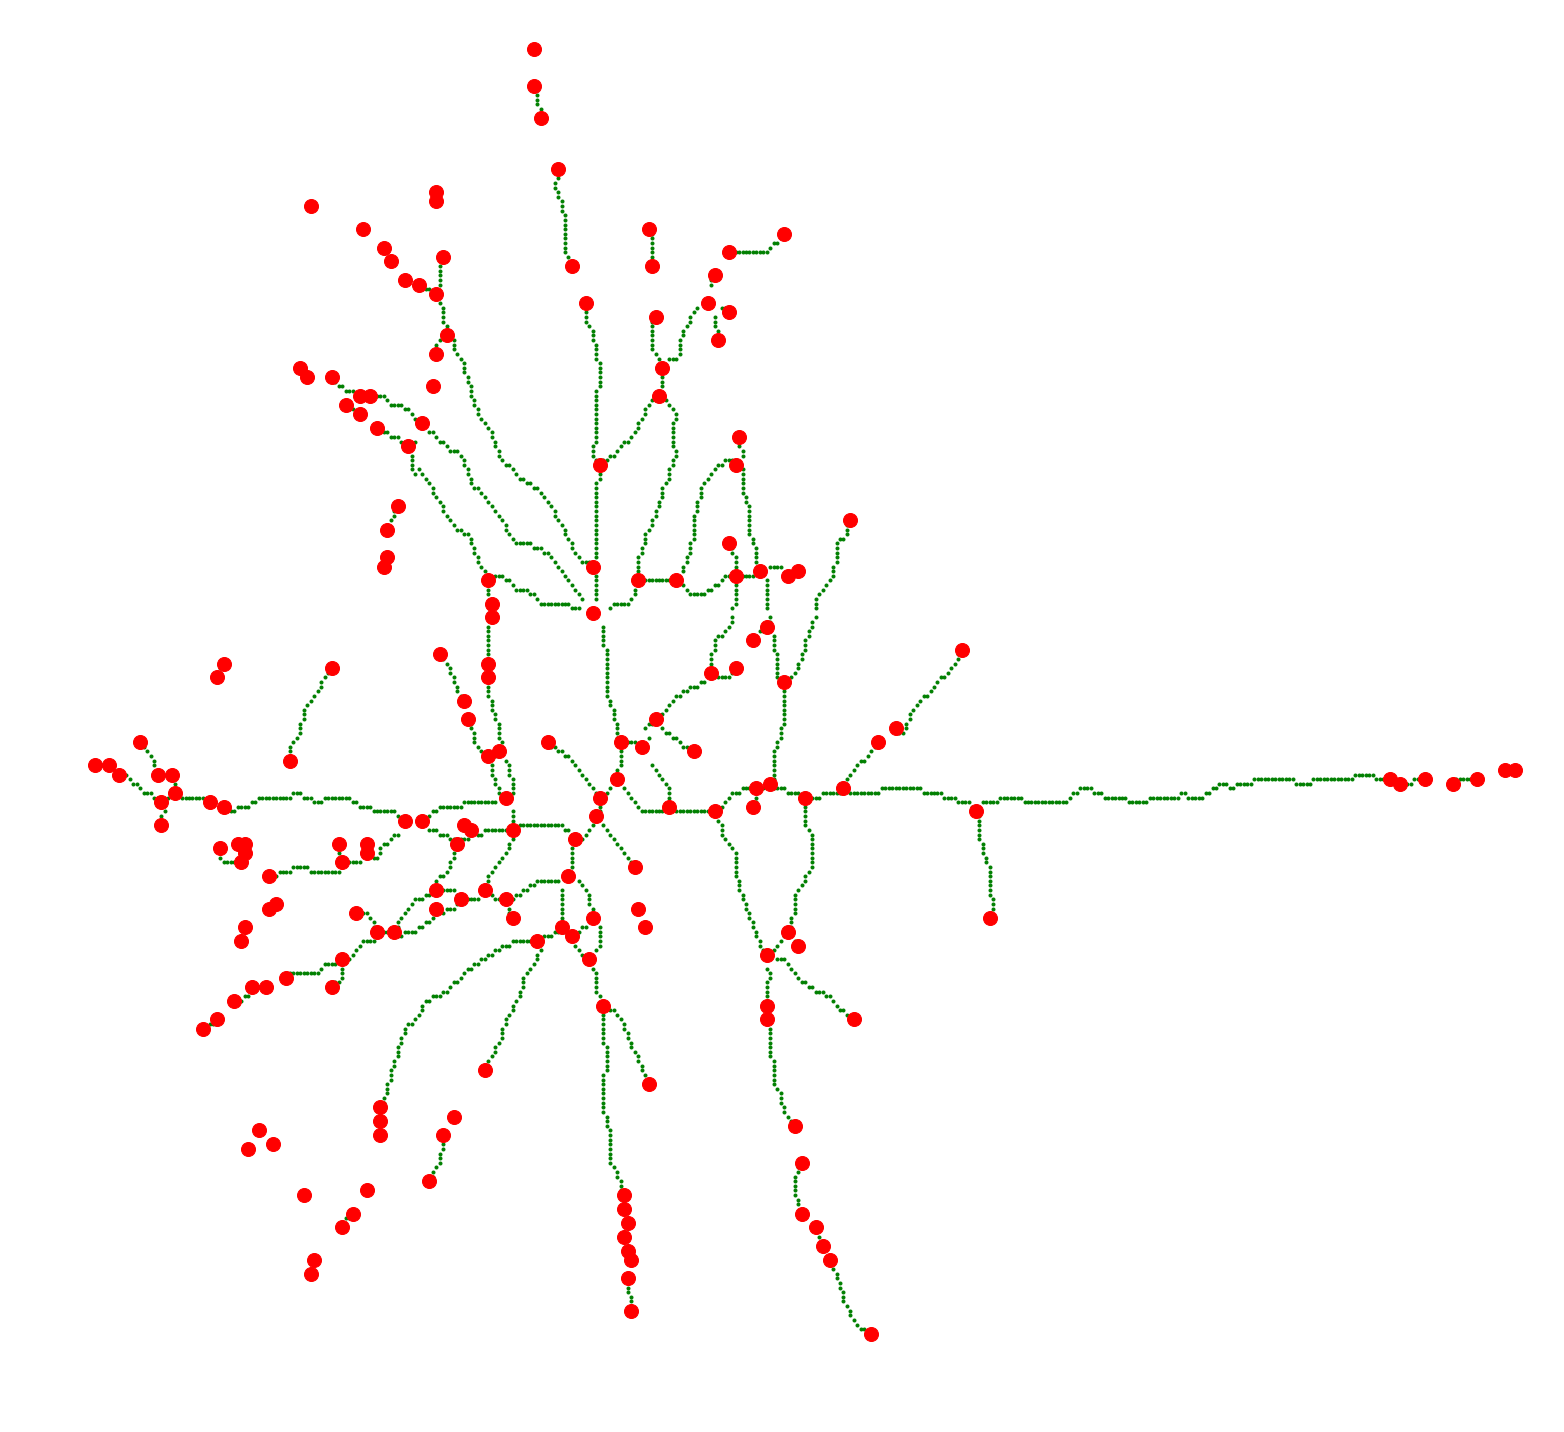
\includegraphics[height=2in]{benchImages/grupo1-Porta10-5b-AVG_partialCleaned-graph-thick.png}
        \caption{Grafo base para la individualizaci\'on automatizada de filamentos.}
        \label{fig:Porta10-5b-graph}
    \end{subfigure}
    \caption{Individualizaci\'on manual de una neurona. a) Imagen de ... obtenida al realizar la proyecci\'on del eje Z bajo el criterio de valor m\'aximo de p\'ixeles. b) Representaci\'on mediante colores de los filamentos de la neurona, representando el ax\'on y las dendritas. d) Grafo de X aristas extra\'ido a partir de la individualizaci\'on manual.}
    \label{fig:Porta10-5b}
\end{figure*}


%Porta18-3a1
\begin{figure*}[h!]
    \centering
    \begin{subfigure}[t]{0.49\textwidth}
        \centering
        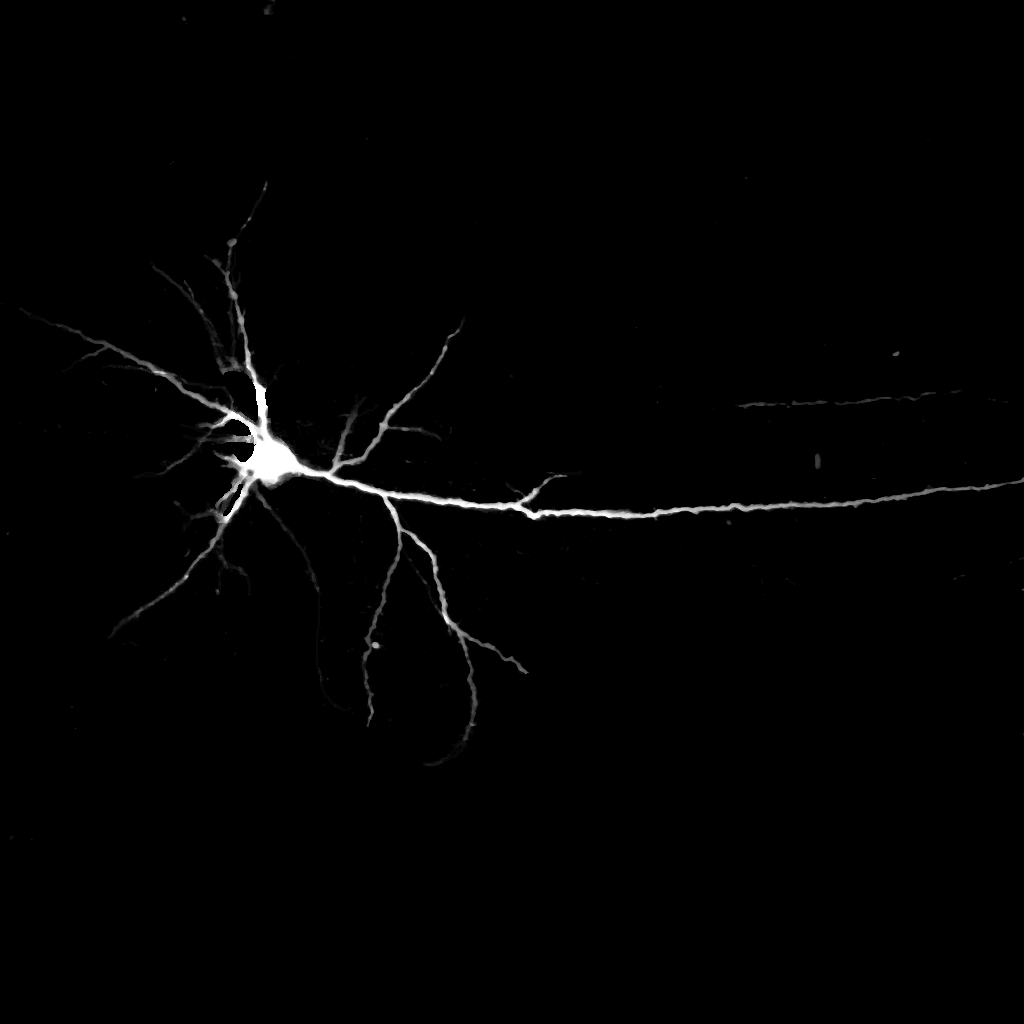
\includegraphics[height=1.9in]{benchImages/grupo2-Porta18-3a1-AVG-cleaned.png}
        \caption{Imagen de una neurona.}
        \label{fig:Porta18-3a1-og}
    \end{subfigure}
    ~ 
    \begin{subfigure}[t]{0.49\textwidth}
        \centering
        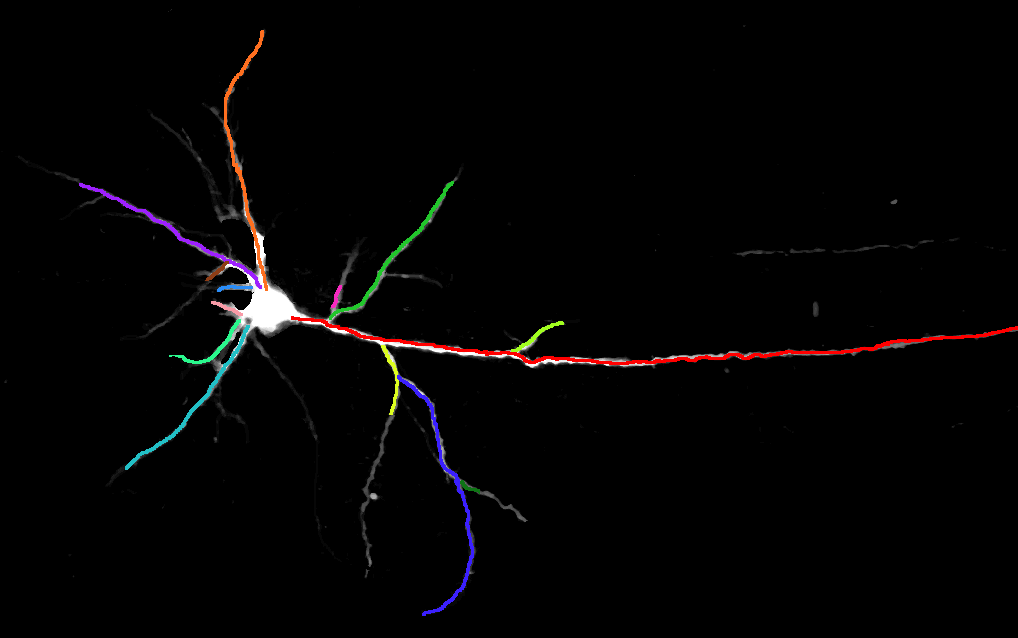
\includegraphics[height=1.9in]{benchImages/grupo2-Porta18-3a1-AVG-cleaned-colorCoded.png}
        \caption{Filamentos manualmente individualizados por un experto.}
        \label{fig:Porta18-3a1-gt}
    \end{subfigure}
    \vskip\baselineskip
    \begin{subfigure}[t]{0.5\textwidth}
        \centering
        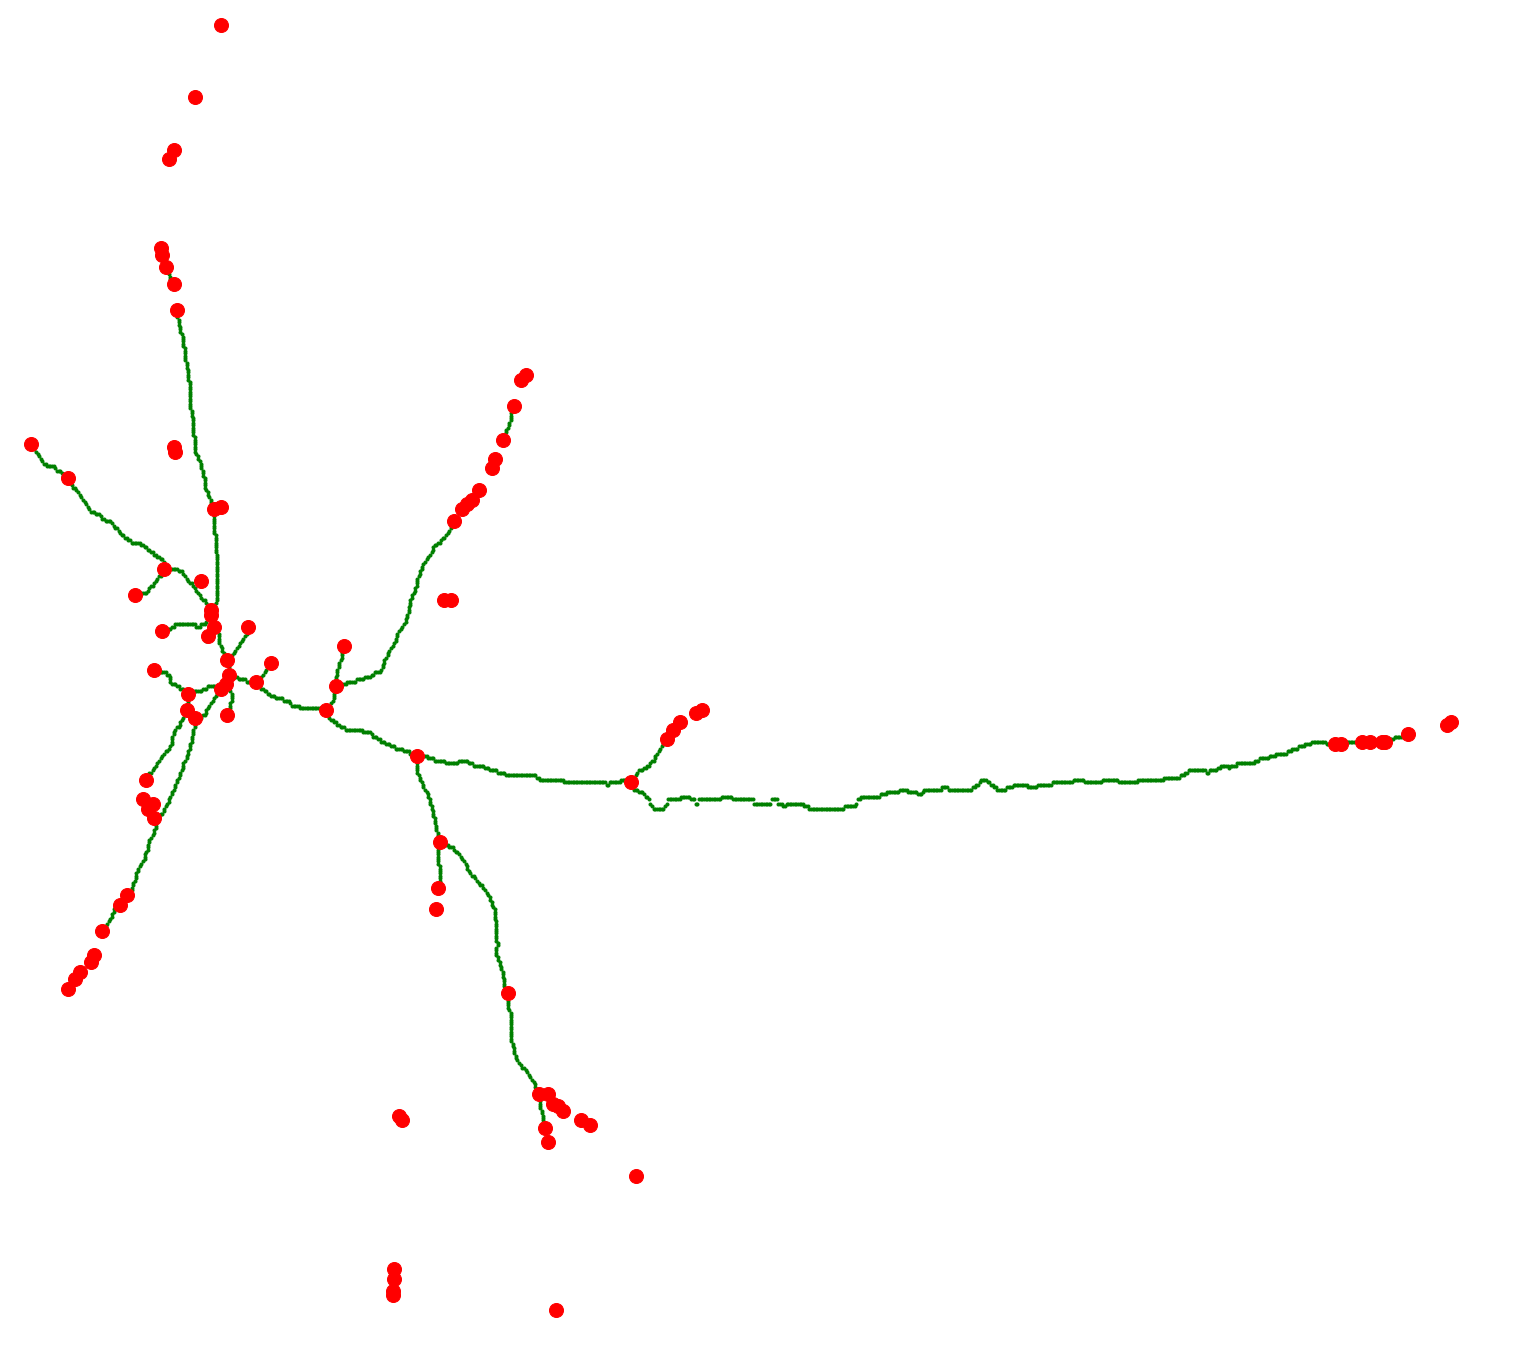
\includegraphics[height=2in]{benchImages/grupo2-Porta18-3a1-AVG-cleaned-graph-thick.png}
        \caption{Grafo base para la individualizaci\'on automatizada de filamentos.}
        \label{fig:Porta18-3a1-graph}
    \end{subfigure}
    \caption{Individualizaci\'on manual de una neurona. a) Imagen de ... obtenida al realizar la proyecci\'on del eje Z bajo el criterio de valor m\'aximo de p\'ixeles. b) Representaci\'on mediante colores de los filamentos de la neurona, representando el ax\'on y las dendritas. d) Grafo de X aristas extra\'ido a partir de la individualizaci\'on manual.}
    \label{fig:Porta18-3a1}
\end{figure*}